% noTE:
% cite EKF thesis
 
 
\documentclass[letterpaper, 10 pt, conference]{ieeeconf}
\IEEEoverridecommandlockouts
\overrideIEEEmargins

% ------------------------------------------------------------------------
% Packages
% ------------------------------------------------------------------------
\usepackage{graphicx} 
\usepackage[cmex10]{amsmath} 
\usepackage{array}
\usepackage[tight,footnotesize]{subfigure} 
\usepackage{amssymb}
\usepackage{bm} 
\usepackage{algorithm} 
\usepackage{algorithmic}
\usepackage{enumerate} 
\usepackage{multirow} 
\usepackage[noadjust]{cite}
\usepackage[usenames,dvipsnames]{color}
\usepackage{epstopdf}

% ------------------------------------------------------------------------
% Figure Path
% ------------------------------------------------------------------------
\graphicspath{{./fig/}}

% ------------------------------------------------------------------------
% Theorem Related
% ------------------------------------------------------------------------
\newtheorem{thm}{Theorem}[section] \newtheorem{cor}[thm]{Corollary}
\newtheorem{prob}[thm]{Problem} \newtheorem{lem}[thm]{Lemma}
\newtheorem{prop}[thm]{Proposition} \newtheorem{defn}[thm]{Definition}
\newtheorem{rem}[thm]{Remark} \newtheorem{example}[thm]{Example}

% ------------------------------------------------------------------------
% Abbreviation for Math
% ------------------------------------------------------------------------
\newcommand{\set}[1]{\{#1\}} \newcommand{\norm}[1]{\|#1\|}
\newcommand{\mc}[1]{\mathcal{#1}} \newcommand{\mb}[1]{\mathbf{#1}}
\newcommand{\mt}[1]{\mathtt{#1}}
\newcommand{\Cov}{\operatorname{Cov}}
\newcommand{\E}{\mathbb{E}}
%\newcommand{\E}{\operatorname{E}}
\newcommand{\Var}{\operatorname{Var}}
\newcommand{\Corr}{\operatorname{Corr}}
\newcommand{\I}{\mc{I}}
\newcommand{\Real}{\mathbb{R}} 
\newcommand{\Integer}{\mathbb{Z}}
\newcommand{\diag}{\text{diag}}
\newcommand{\ZPlus}{\mathbb{Z}_{>0}} 
\newcommand{\RPlus}{\mathbb{R}_{>0}} 
\newcommand{\GP}{\mathcal{GP}}
\newcommand{\M}{M}
\newcommand{\Normal}{\mc{N}}
\newcommand{\N}{\mc{N}}
\newcommand{\V}{\mc{V}}
\newcommand{\A}[1]{\mc{A}_{#1}}
\newcommand{\C}{\gamma}
\newcommand{\removed}[1]{}%{\color{Fuchsia} #1}}
\newcommand{\changed}[2]{{\color{blue} #2}}
\newcommand{\added}[1]{{\color{Fuchsia} #1}}
\newcommand{\comment}[1]{}
\newcommand{\f}[2]{f_{#1}\left(#2\right)}
\newcommand{\D}[2]{\mc{D}_{#2}}
\newcommand{\Di}[3]{\mc{D}^{(#1)}_{#2:#3}}
\newcommand{\R}[2]{\mc{R}_{#1:#2}}
\renewcommand{\P}[1]{\mc{P}_{#1}}
%\renewcommand{\sum}[1]{\textsc{SUM}\left(#1\right)}
%\renewcommand{\Sigma}{\Lambda}
\newcommand{\betat}[1]{\beta_{#1}}
\newcommand{\thetal}[1]{\theta}
\newcommand{\q}[1]{{q_{#1}}}
\newcommand{\qi}[2]{q^{(#1)}_{#2}}
\newcommand{\tildez}[1]{{\tilde{z}_{#1}}}
\newcommand{\tildeq}[1]{{\tilde{q}_{#1}}}
\newcommand{\tildezi}[2]{{\tilde{z}_{#2}^{[#1]}}}
\newcommand{\tildeqi}[2]{{\tilde{q}_{#2}^{[#1]}}}
\newcommand{\y}[1]{{y_{#1}}}
\newcommand{\x}[1]{{x_{#1}}}
\newcommand{\z}[1]{{z_{#1}}}
\newcommand{\w}{W}
\newcommand{\e}{E}
\newcommand{\K}{\Sigma}
% ------------------------------------------------------------------------
% Begin Document
% ------------------------------------------------------------------------
\begin{document}

% ------------------------------------------------------------------------
% Front Matter
% ------------------------------------------------------------------------
\title{\LARGE \bf Fully Bayesian Simultaneous Localization and Spatial Prediction using Gaussian Markov Random Fields (GMRFs)}

\author{Mahdi~Jadaliha, Do Huan and Jongeun~Choi
 \thanks{Mahdi Jadaliha and Do Huan are with the Department of Mechanical Engineering,
 Michigan State University, East Lansing, MI 48824, USA. E-mail:
 jadaliha@msu.edu.}
 \thanks{Jongeun Choi is with the Department of Mechanical
 Engineering and the Department of Electrical and Computer Engineering, Michigan
 State University, East Lansing, MI 48824, USA. E-mail:
 jchoi@egr.msu.edu.}}
\maketitle
\thispagestyle{empty}
\pagestyle{empty}

\begin{abstract}
This paper investigates a fully Bayesian way to solve the simultaneous localization and spatial prediction (SLAP) problem using a Gaussian Markov random field (GMRF) model. The objective is to simultaneously localize robotic sensors and predict a spatial field of interest using sequentially obtained noisy observations collected by robotic sensors. The set of observations consists of the observed uncertain poses of robotic sensing vehicles and noisy measurements of a spatial field. To be flexible, the spatial field of interest is modeled by a GMRF with uncertain hyperparameters. We derive an approximate Bayesian solution to the problem of computing the predictive inferences of the GMRF and the localization, taking into account observations, uncertain hyperparameters, measurement noise, kinematics of robotic sensors, and uncertain localization. 
The effectiveness of the proposed algorithm is illustrated by simulation results.
\end{abstract}

% ------------------------------------------------------------------------
%
% ------------------------------------------------------------------------
\section{Introduction}

 The simultaneous  localization and mapping (SLAM) problem  is important to be solved    for  a robot  to explore  an unknown environment under localization uncertainty \cite{dissanayake2001solution}. 
%
%While exploring the environment, the robot seeks to predict a map thereof, and at the same time it wishes to localize itself using its map. SLAM appeals to engineers for solutions in two different cases. One might be interested in building a precise map, or others might seek to maintain an accurate sense of mobile robot's location. SLAM serves both of these purposes \cite{dissanayake2001solution, guivant2001optimization,montemerlo2003fastslam, murphy1999bayesian}. 
%
The variations of the SLAM problem are surveyed and categorized with different perspectives in \cite{thrun2008simultaneous}.
In general, most SLAM problems have strong geometric models \cite{leonard1991simultaneous,dissanayake2001solution, guivant2001optimization,montemerlo2003fastslam,murphy1999bayesian,thrun2008simultaneous}. For example, a robot learns the locations of the landmarks while localizing itself using triangulation algorithms. Such geometric models could be classified in two groups, viz., 
%\begin{enumerate}
%	\item 
	a sparse set of features which can be individually identified, often used in Kalman filtering methods \cite{dissanayake2001solution}, and 
	%\item 
	a dense representation such as an occupancy grid, often used in particle filtering methods \cite{grisettiyz2005improving}.
%\end{enumerate}

In contrast to the SLAM problem with popular geometrical models, there is a growing number of practical scenarios in which no such geometric model exists. Consider localization using various spatially distributed (continuous) signals such as distributed wireless Ethernet signal strength \cite{ferris2007wifi}, or multi-dimensional magnetic fields \cite{vallivaara2010simultaneous}. Underwater autonomous gliders for ocean sampling cannot find usual geometrical models from measurements of environmental variables such as pH, salinity, and temperature \cite{leonard:2007}. Furthermore, there are reasons to avoid the geometric model as well, even when a geometric model does exist.
 {Such cases may include:
 1)  the difficulty of reliably extracting sparse, stable features,
 2)  the ability to use all  sensory data directly  rather than a relatively small amount of abstracted discrete information obtained from feature extraction algorithms, and 
 3)  high computational and storage costs of dealing with dense features.}
 


Motivated by the aforementioned situations, in this paper, we consider scenarios without geometric models and tackle the problem of simultaneous localization and prediction (SLAP) of a spatial field. %Emphasizing on not having a geometric model, our problem will be referred to as SLAP for the rest of the paper.

%
%
% 
 
 
 Nonparametric modeling and prediction techniques for random fields have been exploited for mobile robotic sensors \cite{lynch:2008, leonard:2007,choi:2009,cortes:2009,Xu2011sequential}. Random fields such as Gaussian processes and Gaussian Markov random fields (GMRFs)  \cite{cressie:1986,rasmussen:2006} have been frequently used for mobile sensor networks to statistically model physical phenomena such as harmful algal blooms, pH, salinity, temperature, and wireless signal strength e.g., \cite{krause:2008,xu:2011b,graham:2009}.

 {
 The recent research efforts that are closely related to our problem are summarized as follows.
In \cite{jad2012gaussian}, the authors  formulated Gaussian process regression under uncertain localization. In \cite{jadaliha2012efficient},  the authors used a GMRF with uncertain hyperparameters and  tackled a problem of prediction of the random field  under  localization uncertainty.
However, kinematics or dynamics of the sensor vehicles were not incorporated in \cite{jad2012gaussian,jadaliha2012efficient}.}
 In \cite{brooks2008gaussian},  Gaussian process regression was used to model geo-referenced sensor measurements (obtained from a camera). After training with  data including noisy measurements and their exact sampling positions, a maximum likelihood estimator was used to find the best match for  the  location of  each of newly sampled measurements. However, this was not SLAM since the training step has to be performed {\em a priori} for a given environment \cite{brooks2008gaussian}.
In \cite{kemppainen2010near,vallivaara2010simultaneous},  Gaussian process regression was also used to implement SLAM using a magnetic field and the  feasibility of such approaches were shown 
experimentally.
The work in \cite{o2009contextual}  used laser range-finder data to probabilistically classify the
 robot's environment into a region of occupancy. It  provides a continuous representation of robot's surroundings by employing a Gaussian process.
In \cite{ferris2007wifi},  so called a WiF-SLAM problem was solved using a Gaussian process latent variable model (GP-LVM). 
%It was shown that GP-LVMs in combination with a dynamic model could reconstruct connectivity graphs and GP sensor models that can be used for WiFi localization. 
However, the accurately known training data and the independence across the dimensions and instantiations of the data were assumed in \cite{ferris2007wifi}, which may  not be practical.
To the best of our knowledge, most work related to our SLAP problem did not address uncertainties in the hyperparameters of the Gaussian process in a fully Bayesian way. In most of the previous work, the hyperparamters in the model were estimated offline {\em a priori}.

 
 In this paper, we   formulate the simultaneous localization and spatial prediction (SLAP) problem, in order to simultaneously localize robotic sensors and predict a spatial random field of interest using sequentially obtained noisy observations collected by robotic sensors. The set of observations consists of the observed uncertain poses of robotic sensing vehicles and noisy measurements of a spatial field.  To be flexible, the spatial field of interest is modeled by a GMRF with uncertain hyperparameters. We then derive an approximate Bayesian solution to the problem of computing the predictive inferences of the GMRF and the localization, taking into account observations, uncertain hyperparameters, measurement noise, kinematics of robotic sensors, and uncertain localization. The effectiveness of the proposed algorithm is illustrated by simulation results.

 

Standard notation will be used throughout the paper. Let $\Real$ and $\Integer_{>0}$ denote, respectively, the sets of real and positive integer numbers. The collection of $n$ number of $m$ dimensional vectors $\{ q_i \in \Real^m \, |\, i =1, \cdots, n \}$ can be defined by $q:=\text{col} \left (q_1, \cdots, q_n \right ) \in \Real^{nm}$ using the notation $\text{col} (\cdot)$.
The operators of expectation and covariance matrix are denoted by $\E$ and $\Cov$, respectively. A random vector $x$, which has a multivariate normal distribution of mean vector $\mu$ and covariance matrix $\Sigma$, is denoted by $x \sim \mc{N}(\mu,\Sigma)$. For given ${G}=\set{c,d}$ and ${H}=\set{1,2}$, the multiplication between two sets is defined as ${H} \times {G}= \set{(1,c), (1,d),(2, c),(2,d)}$. 
%The probability density function of observing $x$ for the random variable $X$ will be denoted by $\f{X}{x}$. 
%When it is obvious, $\pi\left(x\right)$ or $\pi\left(X\right)$ will be used for $\f{X}{x}$ for notational simplicity. 
%The notation of the discrete probability distribution and its short notation will be defined in a similar way. We adopt this short notation, which is often used in the machine learning community. 
Other notation will be explained in due course.

 % ------------------------------------------------------------------------
% ------------------------------------------------------------------------
%\section{Preliminaries}

%
%\section{Sequential Bayesian inference with a Gaussian process}\label{sec:SeqBay}
%In the following discussion, we formulate the SLAP problem in a sequential form considering the random field as a Gaussian process over a compact continuum domain $\mc{S}_c$. 
% 
%
%
%Consider $x: = \text{col} \left(x^{[1]},\cdots,x^{[p]}\right) \in \mc{S}^p_c$ as a collation of $p$ locations in the surveillance region. The collection of the realized values of the random field at $x$ is denoted by $z\left(x\right) := \text{col} \left( z\left(x^{[1]}\right),\cdots,z\left(x^{[p]}\right)\right )$. Let $N$ be the \changed{}{robotic vehicles'} number\changed{}{, and} denote robotic vehicles' sampling positions and their control inputs at time~$t$ by $q_t := \text{col} \left(q_t^{[1]},\cdots,q_t^{[N]}\right) \in \mc{S}^{ N}_c$ and $u_t := \text{col} \left(u_t^{[1]},\cdots,u_t^{[N]}\right)$, respectively. The observed positions of the robots and values of the random field are 
%corrupted by noises as follows.
%\begin{equation}
%\begin{split}
%\tilde{q}_t & = q_t + e_t,\\ 
%\tildez{t} &= z\left(q_t\right) + \epsilon_t,
%\end{split}
%\label{eq:observed_formulas}
%\end{equation}
%where $e_t$ and $\epsilon_t$ are additive noises.
%We denote the collections of cumulative robots' locations, cumulative observations, and cumulative control inputs from time $1$ to time $t$, respectively, by $\tilde{q}_{1:t} := \text{col} \left(\tilde{q}_{1},\cdots,\tilde{q}_{t} \right) \in \mc{S}^{ N t}_c$, $\tildez{1:t} := \text{col} \left(\tildez{1},\cdots,\tildez{t}\right) \in \Real^{N t}$, and $u_{1:t} := \text{col} \left(u_{1},\cdots,u_{t}\right).$ % \in \Real^{N t}$. 
%Furthermore, we define the cumulative data set by $\D{1}{t}:=\set{\tilde{z}_{1:t},\tilde{q}_{1:t}}$. 
%
%
%
%
%Now we introduce the evolution of the robots over the discrete time index $t$ as follows.
%\begin{equation}
%\begin{split}
%\q{t+1} &= \q{t} +F_t u_t + w_t, \\
%%\z{t}\left(x\right) &= \z{t - 1}\left(x\right) + \varsigma_{t - 1}\left(x\right),
%\end{split}
%\label{eq:iterative_formulas}
%\end{equation}
%\changed{}{
%where $u_t$, $w_t$, and $F_t$ are the control input, the system noise, and the input matrix, respectively. }
%The general motion description in \eqref{eq:iterative_formulas} can be viewed as a discretized version of the continuous time vehicle dynamics. We will use specific vehicle dynamics in the next section to be more specific. 
%
%In this section, we consider a static random field at a position $x$ given by a Gaussian process with an uncertain hyperparameter vector $\theta$:
%\begin{equation}
%%\z{t}\left(x\right)=
%z(x) \sim \mathcal{GP} (\mu(x;\theta), \mathcal{K}(x, x'; \theta) ), % = z \left(x\right),
%\label{eq:iterative_formulas2}
%\end{equation}
%where $\mu(x;\theta)$ and $\mathcal{K}(x, x'; \theta)$ are mean and covariance functions.
%Assume that at time $t \in \Integer_{>0}$, a new set of observations $\set{\tilde{z}_t,\tilde{q}_t}$ is collected by a network of robotic vehicles at \changed{its}{their} current configuration $\q{t}$. 
%We now state our SLAP problem with a Gaussian process over a continuum space.
%
%
%\begin{prob}\label{prob:certain0}
%Given aforementioned assumptions and models in \eqref{eq:observed_formulas}, \eqref{eq:iterative_formulas}, and \eqref{eq:iterative_formulas2}, our SLAP problem is to find the conditional probability density function of $z(x)$ given $\D{1}{t}$. 
%\end{prob}
%
%
%In what follows, we present our approach for the solution to Problem~\ref{prob:certain0}. \changed{}{Assume $\beta$, $\gamma$, $\nu$, $\rho$, $\vartheta$, $\varsigma$, and $\phi$  are a realization of the random variables  $\theta$, $q_t$, $q_{t-1}$, $\tilde{z}_t$, $z(q_t)$, $z(x)$, and $\tilde{q}_t$, respectively.}
%
%From \eqref{eq:iterative_formulas}, the conditional probability density function of $\theta,\q{t}|\D{0}{t - 1}$ is formulated as follows. 		
%\begin{equation}
%\begin{split}
%		&\f{\theta,\q{t}|\D{0}{t - 1}}{\beta,\gamma|\D{0}{t - 1}} = \\
%		&\int \int \f{\theta,\q{t - 1}|\D{0}{t - 1}}{\beta,\nu|\D{0}{t - 1}} 
%		\f{w_{t-1}}{\gamma - \nu - F_{t} u_{t-1}} d\nu.
%		\end{split}
%\label{eq:thetaqgivenD}
%\end{equation}
%
% %The probability density function of ${z}_{t}|\theta,\q{t},\D{1}{t-1}$ can be obtained by using \eqref{eq:iterative_formulas2} as follows.	
%%\begin{equation}
%					%\f{z_{t}\left(x\right)|\theta,\D{1}{t-1}}{\varsigma|\beta,\D{1}{t-1}} = 
%					%\int{\f{z_{t-1}\left(x\right)|\theta,\D{}{t-1}}{\lambda|\beta,\D{}{t-1}} 
%					%\f{\varsigma_{t-1}\left(x\right)}{\varsigma - \lambda} d\lambda}.		 
%%\label{eq:z_tgiventhtaandq}
%%\end{equation}				
%					%
%Using \eqref{eq:observed_formulas}, the probability density function of the observed data $\tilde{z}_{t}$ at the possible sampling position $\q{t}$ and the hyperparameter vector $\theta$ is given by the formula
%\begin{equation}
%\begin{split}
%					&\f{\tilde{z}_{t}|\theta,\q{t},\D{1}{t-1}}{\rho|\beta,\gamma,\D{1}{t-1}} = 	\\
%					& \quad \quad \quad \int{\f{z\left(q_t\right)|\theta,\D{1}{t-1}}{\vartheta|\beta,\D{1}{t-1}} 	\f{\epsilon_t}{\rho - \vartheta} d\vartheta}.
%\end{split}
%\label{eq:ztildagiventhetaandq}
%\end{equation}
%The posterior probability density function of $z\left(x\right)|\theta,q_t,\D{1}{t}$ is equivalent to that of $z\left(x\right)|\theta,q_t,\tilde{z}_t,\D{1}{t-1}$, which can be obtained as follows.
%\begin{equation}
%\begin{split}
%&\f{z\left(x\right)|\theta,q_t,\tilde{z}_t,\D{1}{t-1}}{\varsigma|\beta,\gamma,\rho,\D{1}{t-1}} = \\
%&\quad \quad\quad \quad\quad \quad \frac{\f{z\left(x\right),\tilde{z}_t|\theta,q_t,\D{1}{t-1}}{\varsigma,\rho|\beta,\gamma,\D{1}{t-1}}}{\f{\tilde{z}_{t}|\theta,\q{t},\D{1}{t-1}}{\rho|\beta,\gamma,\D{1}{t-1}}},
%\end{split}
%\label{eq:}
%\end{equation}	
%where the density function of $z\left(x\right),\tilde{z}_t|\theta,q_t,\D{1}{t-1}$ is given by Gaussian process regression using \eqref{eq:iterative_formulas2}.
%The joint probability density function of the sampling position and the hyperparameter vector using the observed data up to time $t$ can be computed by the following relationship. 
%\begin{equation}
%\begin{split}
%&\f{\theta,\q{t} |\D{}{t}}{\beta, \gamma |\D{}{t}} \propto \\
%&				 	\f{\theta, q_{t} |\D{}{t - 1}}{\beta,\gamma|\D{}{t - 1}}
%					\f{\tilde{q}_t,\tilde{z}_t|\theta,\q{t},\D{0}{t-1}}{\phi,\rho|\beta, \gamma,\D{0}{t-1}},					
%\end{split}
%\end{equation}
%where 
%\[					
%\begin{split}
%& \f{\tilde{q}_t,\tilde{z}_t|\theta,\q{t},\D{0}{t-1}}{\phi,\rho|\beta, \gamma,\D{0}{t-1}} =\\
%& \quad \quad\quad \quad\quad \quad \f{\tilde{q}_t|q_t}{\phi|\gamma}
%					 \f{\tilde{z}_t|\theta,\q{t},\D{0}{t-1}}{\rho|\beta, \gamma,\D{0}{t-1}},\\					
%&\f{\tilde{q}_t|q_t}{\phi|\gamma} = \f{e_t}{\phi-\gamma}.
%					\end{split}
%					\]
%									
%				 	
%Finally, the probability density functions of the sampling positions, the hyperparameters, and the random field conditional on cumulatively measured data up to time $t$, are obtained by marginalizing uncertainties as \changed{}{the following.}
%\begin{equation}
%\begin{split}
%					&\f{ \q{t}|\D{0}{t}}{ \gamma|\D{0}{t}} = \int \f{ \theta, \q{t} |\D{}{t}}{\beta, \gamma |\D{}{t}} d\beta, \\
%					&\f{\theta |\D{0}{t}}{\beta |\D{0}{t}} = \int \f{\theta, \q{t} |\D{}{t}}{\beta, \gamma |\D{}{t}} d\gamma, \\
%					&\f{z\left(x\right)|\theta, \D{}{t}}{\varsigma|\beta, \D{}{t}} = \\
%					&\frac{1}{\f{\theta |\D{}{t}}{\beta |\D{}{t}}} \int \f{z\left(x\right)|\theta,\q{t}, \D{}{t}}{\varsigma|\beta, \gamma, \D{}{t}} \f{\theta, \q{t} |\D{}{t}}{\beta, \gamma |\D{}{t}} d\gamma, \\
%					&\f{z\left(x\right)| \D{}{t}}{\varsigma|\D{}{t}} = \int \f{z\left(x\right)|\theta, \D{}{t}}{\varsigma|\beta, \D{}{t}} \f{\theta |\D{}{t}}{\beta |\D{}{t}} d\beta. 
%\end{split}
%\label{eq:marginalizeddensitiy}
%\end{equation}
% 
%\begin{rem}
%Unfortunately, the integrals in \eqref{eq:thetaqgivenD}, \eqref{eq:ztildagiventhetaandq}, \eqref{eq:marginalizeddensitiy} do not have closed form solutions. In addition, \eqref{eq:thetaqgivenD} cannot be computed in a fixed time, since we need to recalculate $\f{\theta,\q{\tau}|\D{0}{t - 1}}{\beta,\nu|\D{0}{t - 1}}$ for $\tau \in \set{1, \cdots, t-1}.$ Thus, this exact recursive Bayesian solution is neither analytical nor computationally tractable. 
%\changed{}{In addition, approximation techniques} such as MCMC sampling and Laplace approximations may not be scalable as the number of observations increases. In this paper, therefore, we consider a discretized version of this problem and its solution, which are provided in the subsequent section. 
%\end{rem} 
% 
%

\section{Sequential Baysian inference with a GMRF} \label{sec:Sequential Baysian}
In this section,  we define  a GMRF model in detail, formulate the problem, and provide its solution. 


\subsection{Gaussian processes and Gaussian Markov random fields}\label{sec:GP-GMRF}
In this section, we briefly introduce a GMRF as a discretized Gaussian process on a lattice.
Consider a Gaussian process: $z(q) \sim \mc{GP}(\mu, \Sigma),$ where $\mu$ is the mean vector, and $\Sigma \in \Real^{n \times n}$ is the covariance matrix. We discretize the compact domain $\mc{S}_c := [0 ~ x_{max}] \times [0 ~ y_{max}]$ into $n$ spatial sites $\mc{S}:= \set{s^{[1]},\cdots,s^{[n]}} \subset \Real^d$, where $n = h x_{max} \times h y_{max}$. $h$ will be chosen such that $n \in \ZPlus$.
Note that $n \rightarrow \infty$ as $h \rightarrow \infty.$ The collection of realized values of the random field in $\mc{S}$ is denoted by $z := (z^{[1]},\cdots,z^{[n]})^T \in \Real^{n}$, where $z^{[i]} :=z(s^{[i]})$.

%We will  use a short notation $\pi\left(x\right)$ or $\pi\left(X\right)$ for $\f{X}{x}$ and the probability of that $X=x$, i.e., Pr$(X=x)$ whenever it is obvious. 
The prior distribution of $z$ is given by $\Normal(\mu,\Sigma)$. We then  have 
\begin{equation}
 \pi(z) \propto \exp \left( -\frac{1}{2} \left(z - \mu\right)^T \Sigma^{-1} \left(z - \mu\right) \right).
\label{eq:z_prob}
\end{equation}
The $i,j$-th element of $\Sigma$ is defined as $\Sigma^{[ij]} = \Cov(z^{[i]},z^{[j]}).$ %=\K(z^{[i]},z^{[j]})$.
The prior distribution of $z$ can be written by a precision matrix $Q=\Sigma^{-1}$, i.e., $z \sim \Normal(\mu,Q^{-1})$.
%\begin{equation*}
% \pi(z) \propto \exp \left( -\frac{1}{2} z^T Q_0 z \right),
%\end{equation*}
%where $Q_0 = \Sigma_0^{-1} \in \Real^{n \times n}$ is the precision matrix. 
This can be viewed as a discretized version of the Gaussian process (or a GMRF) with a precision matrix $Q$ on $\mc{S}.$ Note that $Q$ of this GMRF is not sparse. However, a sparse version of $Q$, i.e., $\hat Q$ with local neighborhood that can represent the original Gaussian process can be found, for example, making $\hat Q$ close to $Q$ in some norm \cite{rue:2002,cressie:2008,hartman:2008}. 
This approximate GMRF will be computationally efficient due to the sparsity of $\hat Q$. 
In our simulation study, we will use a GMRF with a sparse precision matrix that represents a Gaussian process precisely as shown in \cite{lindgren:2011,jadaliha2012efficient}. However, any parameterization of $\mu_\theta$ and $Q_\theta$, where $\theta$ is the hyperparameter vector, can be used. 
%For our main problems, we will use a GMRF with a sparse precision matrix that represents a Gaussian process precisely.

%
%We assume that we take $N$ noisy measurements $\tilde{z} = (\tilde{z}^{[1]}, \cdots, \tilde{z}^{[N]})^T \in
%\Real^N$ from corresponding sampling locations $q_c = (q_c^{[1]T}, \cdots, q_c^{[N]T})^T
%\in \mc{S}_c^N$. Here, the measurement model is given by
%\begin{equation*}
% \tilde{z}^{[i]} := \tilde{z}(q_c^{[i]}) = z(q_c^{[i]}) + \epsilon^{[i]}, \forall i = 1, \cdots, N
%\end{equation*}
%where $\epsilon^{[i]} \overset{\text{i.i.d.}}{\sim} \Normal(0,\sigma_{\epsilon}^2)$ is
%the measurement noise and is assumed to be independent and identically
%distributed (i.i.d.). Using Gaussian process regression, the posterior distribution for $z
%\in \Real^n$ is given by
%\begin{equation}
% \label{eq:posterior-gp}
% z|q_c,\tilde{z} \sim \Normal(\mu,\Sigma).
%\end{equation}
%The predictive mean $\mu \in \Real^n$ and covariance matrix
%$\Sigma \in \Real^{n \times n}$ can by obtained by
%\begin{equation}
% \label{eq:gpr}
% \begin{split}
% \mu = \mu_0 + K^T C^{-1} \left(\tilde{z}-\mu_{\tilde{z}} \right), \quad 
% \Sigma = \Sigma_0 - K^T C^{-1} K,
% \end{split}
%\end{equation}
%where the covariance matrices are defined as $K :=
%\Cov(\tilde{z},z) \in \Real^{N \times n}$, $C :=
%\Cov(\tilde{z},\tilde{z}) \in \Real^{N \times N}$, and $\mu_{\tilde{z}} \in \Real^{N}$ is a known mean vector for $\tilde{z}$.



\subsection{Multiple robotic sensors}
Consider $N$ spatially distributed robots with sensors indexed by $j \in \mc{J} := \set{1,\cdots,N}$ sampling at time $t \in \Integer_{>0}$. Suppose that the sampling time $t \in \ZPlus$ is discrete. 
Recall that the surveillance region is   discretized as a lattice that consists of $n$ spatial sites,  whose set  is denoted by $\mc{S}$. Let $n$ spatial sites in $\mc{S}$ be indexed by $\mc{I}:=\{1, \cdots, n\}$, and $z := \text{col} \left ( z^{[1]},\cdots,z^{[n]} \right ) \in \Real^{n}$ be the corresponding static values of the scalar field at $n$ special sites. 
We denote all robots' locations at time $t$ by $\q{t} = \text{col} \left(\q{t}^{[1]}, \cdots,\q{t}^{[N]}\right) \in \mc{S}^N$, the observations made by all robots at time $t$ by $\tildez{t} = \text{col} \left(\tildezi{1}{t},\cdots,\tildezi{N}{t}\right) \in \Real^N$, and the observed states of all robots at time $t$ by $\tildeq{t} = \text{col} \left( {\tildeqi{1}{t}},\cdots,\tildeqi{N}{t}\right)$. $\tilde{q}_t$ and $\tilde{z}_t$ are noisy observations of $q_t$ and $z$, respectively. At time $t$, robot~$j$ takes a noise corrupted measurement at its current location $\q{t}^{[j]} = s^{[i]} \in \mc{S}, \forall j \in \mc{J}, i \in \mc{I}$, viz.,
\begin{equation}
 \tildezi{j}{t}= z^{[i]} + \epsilon_{t}^{[j]}, 
	\label{eq:z_noise}
\end{equation}
where the measurement errors $\{\epsilon_{t}^{[j]} \}$ are assumed to be the 
 independent and identically distributed (i.i.d.) Gaussian white noise, i.e., $\epsilon_{t}^{[j]}
 \overset{i.i.d.}{\sim} \mc{N}(0,\sigma_{\epsilon}^2)$. The measurement noise level $\sigma_{\epsilon}^2 > 0$ is assumed to be known, and we define $\epsilon_t:=\text{col} \left (\epsilon_t^{[1]},\cdots,\epsilon_t^{[N]} \right ) \in \Real^N$. 

In addition, at time $t$, robot~$j$ takes a noisy observation of its own vehicle position.
\begin{equation}
 \tildeqi{j}{t}= q_{t}^{[j]} + e_{t}^{[j]}, 
 \label{eq:q_noise}
\end{equation}
where the observation errors $\{e_{t}^{[j]} \}$ are distributed by 
$e_{t}^{[j]}
 \overset{i.i.d.}{\sim} \mc{N}(0,\sigma_{e}^2I).$

 The observation noise level $\sigma_{e}^2 > 0$ is assumed to be known, and we define $e_t:= \text{col} \left (e_t^{[1]},\cdots,e_t^{[N]} \right ) \in \Real^{d \times N}$. 

Our models can be represented in the  concise  collective notation.
\begin{equation}
\begin{split}
\tildez{t} &= H_{q_t} z + \epsilon_t,\\
\tilde{q}_t & = L_t q_t + e_t,
\end{split}
\label{eq:y}
\end{equation}
where $L_t$ is the observation matrix for the vehicle states, and $H_{q_\tau} \in \Real^{N \times n}$ is defined by
\begin{equation*}
 H_{q_\tau}^{[ij]} = \left\{
 \begin{array}{ll}
 1, & \text{if $s^{[j]} = q_{\tau}^{[i]}$}, \\
 0, & \text{otherwise}.
 \end{array}
 \right.
\end{equation*}







\subsection{Kinematics of robotic vehicles}
In this section, we introduce a specific model for the motion of robotic vehicles.
Each robotic sensor is modeled by a nonholonomic differentially driven vehicle in a two dimensional domain, i.e., $\mc{S} \in \Real^2$. %The vehicle state consists of a sampling position and a heading. 
In this case, an equation of motion for robot~$i$ % \cite{lawton2003decentralized,
\cite{ren2007consensus} may be given by
\begin{equation}\label{eq:nonholonomic}
\begin{split}
\left[\begin{array}{c}
 \dot q_t^{[1,i]}\\
 \dot q_t^{[2,i]}
 \end{array}
 \right]=
\left[
\begin{array}{c}
u_t^{[i]} \cos \psi_t^{[i]} \\
 u_t^{[i]} \sin \psi_t^{[i]} 
\end{array}
\right] +\beta_t^{[i]},
\end{split}
\end{equation}
where $\set{q_t^{[1,i]}, \, q_t^{[2,i]}}$, $\set{\psi_t^{[i]}}$, $\set{u_t^{[i]}}$, and $\beta_t^{[i]}$ denote the inertial position, the orientation, the linear speed, and the system noise of robot~$i$ in time $t$, respectively. In this case, the kinematics of the vehicle network can be further described in detail as follows. %assuming zero-order hold for the input $u_t$ and continuous integration for the noise $w_t$, to
\begin{equation}
q_{t+1} = q_{t} +F_t u_t + w_t,
\label{eq:discrete_vehicle}
\end{equation}
where $u_t$ is {a known control input and $w_t$ is an i.i.d.} white noise realized by a known normal distribution $\N \left(0,\Sigma_{w_t} \right)$. Assuming that $\{ \psi_t^{[i]} \, | \, \forall i \in \mc{J} \}$ in \eqref{eq:nonholonomic} can be measured precisly, $F_t \in \Real^{2N \times N}$ in \eqref{eq:nonholonomic} is obtained as follows.
\begin{equation*}
F_t = \Delta t \left[ 
\begin{array}{c c c c}
\cos \psi_t^{[1]} & 0 & \cdots & 0 \\
\sin \psi_t^{[1]} & 0 & \cdots & 0 \\
0 & \cos \psi_t^{[2]} & \cdots & 0 \\
0 & \sin \psi_t^{[2]} & \cdots & 0 \\
\vdots & \vdots & \ddots & \vdots \\
0 & 0 & \cdots & \cos \psi_t^{[N]} \\
0 & 0 & \cdots & \sin \psi_t^{[N]} \\
\end{array}
\right],
\end{equation*}
where $\Delta t$ is a sampling time.
We denote the collections of cumulative robots' locations, cumulative observations, and cumulative control inputs from time $1$ to time $t$, respectively, by $\tilde{q}_{1:t} := \text{col} \left(\tilde{q}_{1},\cdots,\tilde{q}_{t} \right) \in \mc{S}^{ N t}_c$, $\tildez{1:t} := \text{col} \left(\tildez{1},\cdots,\tildez{t}\right) \in \Real^{N t}$, and $u_{1:t} := \text{col} \left(u_{1},\cdots,u_{t}\right)  \in \Real^{N t}$. 
 

\subsection{Problem formulation and its Bayesian  predictive inference}\label{subsec:solution}
In this section, we formulate the SLAP problem and  provide its  Bayesian solution.  To be precise, we present 
 the following assumptions A.1-A.5 for the problem formulation.
\begin{description}
\item[A.1] The scalar random field $z$ is generated by a GMRF model which is given by 
$z \sim \Normal(\mu_\theta,Q_\theta^{-1})$, where $\mu_\theta$ and $Q_{\theta}$ are given functions of a hyperparameter vector $\theta$.
\item[A.2] The noisy measurements $\set{ \tilde{z}_{t} }$ and the noisy sampling positions $\set{ \tilde{q}_{t} }$, as in \eqref{eq:y}, are collected by robotic sensors in time~$t = 1, 2, \cdots$.
\item[A.3] The control input $\{ u_{t} \}$ is a known deterministic  vector  at time $t$.
\item[A.4] The prior distribution of the hyperparameter vector $\theta$ is discrete with a support 
 $\Theta = \set{\theta^{(1)},\cdots,\theta^{(L)}}$. 
\item[A.5] The prior distribution of the sampling positions in time $t$, $\pi(\q{t})$, is discrete with a support
 $\Omega(t) = \set{\qi{k}{t}|k \in \mc{L}(t)}$, which is given at time $t$. Here, $\mc{L}(t)=\set{1,\cdots,\C(t)}$ denotes the index in the support and $\C(t)$ is the number of the probable possibilities for $\q{t}$.
\end{description}


%When a new observations $\tilde{z}_{t}$ is collected at current locations $\q{t}$, using Gaussian process regression, the posterior mean and variance for $\z{t}|\theta, \D{1}{t},\q{t}$ are given by
%\begin{equation*}
%\begin{split}
	%\mu_{z_t| \theta,\D{1}{t}, q_t} &= \mu_{\z{t}| \theta,\D{1}{t-1}} + \Sigma_{\z{t}| \theta,\D{1}{t-1}} H_{q_t}^T Q_{\tilde{z}_{t}|\theta,\D{1}{t-1},\q{t}} (\tilde{z}_{t}-\mu_{\tilde{z}_{t}|\theta,\D{1}{t-1},\q{t}}),\\
%\Sigma_{z_t| \theta,\D{1}{t}, q_t} &= \Sigma_{z_t| \theta,\D{1}{t-1}} - \Sigma_{z_t| \theta,\D{1}{t-1}} H_{q_t}^T Q_{\tilde{z}_{t}|\theta,\D{1}{t-1},\q{t}} H_{q_t} \Sigma_{z_t| \theta,\D{1}{t-1}}.
	%\end{split}
%\label{eq:}
%\end{equation*}
%The distribution of $\tilde{z}_{t}| \theta,\D{1}{t-1}, q_t$ is approximated by $\N\left(\mu_{\tilde{z}_{t}| \theta,\D{1}{t-1}, q_t}, Q_{\tilde{z}_{t}| \theta,\D{1}{t-1}, q_t} \right)$. 

\begin{prob}\label{prob:certain}
Consider the assumptions A.1-A.5. Our problem is to   simultaneously find the predictive distributions, means, and variances for both   $z$ and   $q$  conditional on $\D{1}{t}:=\set{\tilde{z}_{1:t},\tilde{q}_{1:t}}$.
\end{prob}




The solution to Problem~\ref{prob:certain} is derived as follows.
The distribution of the GMRF is given by $\pi \left( z|\theta ,\D{0}{t - 1} \right) = \N \left( \mu_{{z}|\theta ,\D{0}{t - 1}}, \Sigma_{{z}|\theta ,\D{0}{t - 1}} \right)$. Recall that the evolution of $q_t$ is given by \eqref{eq:discrete_vehicle} and the input $u_t$ is a known deterministic vector  at time~$t$. Therefore, 
$\pi \left( \q{t}|\D{0}{t - 1} \right)$ can be updated by the Gaussian approximation of $\pi (q_{t-1| \D_{t-1}})$.
\begin{equation}
\begin{split}
& \pi \left( \q{t}|\D{0}{t - 1} \right) \approx \\
& \quad \N\left( \mu_{{\q{t - 1}}|\D{0}{t - 1}} + F_{t-1} u_{t-1},\Sigma_{{\q{t - 1}}|\D{0}{t - 1}} + \Sigma_{w_{t-1}} \right).
\end{split}
\label{eq:prediccted_posib}
\end{equation}
Similarly, $\pi\left({\tilde{z}_{t}|\theta,\D{1}{t-1},\q{t}}\right)$ is updated by the Gaussian approximation of 
$\pi (z | \theta, \D_{t-1})$
as follows.
\begin{equation}
\begin{split}
& \pi\left({\tilde{z}_{t}|\theta,\D{1}{t-1},\q{t}}\right) \approx \\
&\quad \N \left( H_{q_t} \mu_{z| \theta,\D{1}{t-1}}, \Sigma_{\epsilon_t} + H_{q_t} \Sigma_{z| \theta,\D{1}{t-1}} H_{q_t}^T\right).
\end{split}
\label{eq:dis_yt_prd}
\end{equation}

\begin{rem}
%In general the distribution of $\q{t}|\D{0}{t - 1}$ depends on the distribution of $\q{t-1}|\D{0}{t - 1}$ and $w_{t-1}$. Also, the distribution of $\tilde{z}_{t}|\theta,\D{1}{t-1},\q{t}$ depends on the distribution of ${z| \theta,\D{1}{t-1}}$ and $\epsilon_t$. 
For the sake of reducing memory usage and complexity, the distribution of $\q{t}|\D{0}{t - 1}$ and $\tilde{z}_{t}|\theta,\D{1}{t-1},\q{t}$ are approximated by normal distributions.
\end{rem}

The joint distribution $z,\q{t},\theta |\D{0}{t - 1}$ is obtained as follows.
%\changed{}{
\begin{equation}
\begin{split}
&\pi \left( z,\q{t},\theta |\D{0}{t - 1} \right) = \\ &\quad \quad \pi \left( z|\theta,q_t ,\D{0}{t - 1} \right) \pi \left( \theta |q_t, \D{0}{t - 1} \right) \pi \left( \q{t}|\D{0}{t - 1} \right).
\end{split}
\label{eq:26266526}
\end{equation}
%Here we need to approximate $\pi \left( z|\theta,q_t ,\D{0}{t - 1} \right)$ and $\pi \left( \theta |q_t, \D{0}{t - 1} \right)$ by $\pi \left( z|\theta ,\D{0}{t - 1} \right)$ and $\pi \left( \theta |\D{0}{t - 1} \right)$, respectively. Therefore, $\pi \left( z,\q{t},\theta |\D{0}{t - 1} \right)$ is approximated as follows.}
%\begin{equation}
%\pi \left( z,\q{t},\theta |\D{0}{t - 1} \right) \changed{=}{\approx } \pi \left( z|\theta ,\D{0}{t - 1} \right) \pi \left( \theta |\D{0}{t - 1} \right) \pi \left( \q{t}|\D{0}{t - 1} \right).
%\label{eq:26266526}
%\end{equation}
The observation model is given by \eqref{eq:y}, thus the probabilities of the observed data are $\pi \left( \tilde{z}_t|z,\q{t} \right) = \N \left( H_{\q{t}} z,\Sigma_{\varepsilon_t} \right)$ and $\pi \left( \tilde{q}_t|\q{t} \right) = \N \left( L_t \q{t},\Sigma_{e_t} \right)$.
The measured random variables have the following conditional joint distribution,
\begin{equation}
\pi \left( \tilde{z}_t,\tilde{q}_t|z,\q{t},\theta ,\D{0}{t - 1} \right) = \pi \left( \tilde{z}_t|z,\theta,\q{t},\D{}{t-1} \right) \pi \left( \tilde{q}_t|\q{t} \right).
\label{eq:}
\end{equation}

From Bayes' rule, the posterior joint distribution of the scalar field values, the sampling positions, and the hyperparameter vector is given as follows.
\begin{equation}
\pi \left( z,\q{t},\theta |\D{0}{t} \right) = \frac{ \pi \left( \tilde{z}_t, \tilde{q}_t|z,\q{t},\theta ,\D{0}{t - 1} \right) \pi \left(z,\q{t},\theta |\D{0}{t - 1} \right)}{{\pi \left( {{{\tilde z}_t},{{\tilde q}_t}|{D_{t - 1}}} \right)}}.
\label{eq:joint_posterior}
\end{equation}


In addition, $\pi \left(\q{t},\theta |\D{}{t} \right) =\int {\pi \left( z,\q{t},\theta |\D{}{t} \right) dz }$ is given as follows.
\begin{equation}
\begin{split}
 &\int {\pi \left( z,\q{t},\theta |\D{}{t} \right) dz}= \\ 
&\quad \frac{ \pi \left( \tilde{q}_t|\q{t} \right)\pi \left( \theta |q_t, \D{0}{t - 1} \right) \pi \left( \q{t}|\D{0}{t - 1} \right)}{{\pi \left( {{{\tilde z}_t},{{\tilde q}_t}|{D_{t - 1}}} \right)}} \times \\
&\int{\pi \left( z|\theta,q_t ,\D{0}{t - 1} \right) \pi \left( \tilde{z}_t|z,\theta,\q{t},\D{}{t-1} \right) dz},
\end{split}
\label{eq:21132445}
\end{equation}
where $\int{\pi \left( z|\theta,q_t ,\D{0}{t - 1} \right) \pi \left( \tilde{z}_t|z,\theta,\q{t},\D{}{t-1} \right) dz} = \pi\left(\tilde{z}_t|\q{t},\theta,\D{0}{t-1}\right)$,
and $\pi (\tilde{z}_t|\q{t},\theta,\D{0}{t-1})$ is given by \eqref{eq:dis_yt_prd}.

\begin{rem}
From the Bayes' rule, $\pi (\theta |q_t, \D{0}{t - 1})$ is given by $\frac{\pi \left( \theta, q_t| \D{0}{t - 1} \right) }{\pi \left( q_t| \D{0}{t - 1} \right)}$. 
 We can compute $\pi \left( \theta, q_t| \D{0}{t - 1} \right)$ for all the possible combinations of $q_t$ in the previous iteration using \eqref{eq:21132445}. However, for the sake of reducing the computational cost, we approximate $\pi \left( \theta |q_t, \D{0}{t - 1} \right)$ by $\pi \left( \theta |\D{0}{t - 1} \right)$. Therefore, we have 
\begin{equation*}
\begin{split}
&\pi \left(\q{t},\theta |\D{}{t} \right) \approx \\
& \quad \frac{{\pi \left( {{{\tilde q}_t}|{q_t}} \right)\pi \left( {\theta |{D_{t - 1}}} \right)\pi \left( {{q_t}|{D_{t - 1}}} \right)} \pi\left(\tilde{z}_t|\q{t},\theta,\D{0}{t-1} \right)}{{\pi \left( {{{\tilde z}_t},{{\tilde q}_t}|{D_{t - 1}}} \right)}},
\end{split}
\end{equation*}
 \end{rem}

Marginalizing out uncertainties on the possible $\q{t}$ and $\theta$, we obtain the  {following}.
\begin{equation}
\begin{split}
\pi \left( z,\theta |\D{0}{t} \right) &= \sum\limits_{\q{t} \in \Omega(t)} {\pi \left( z,\q{t},\theta |\D{0}{t} \right)},\\
\pi \left( z|\D{0}{t} \right) &= \sum\limits_{\theta \in \Theta} {\pi \left( z,\theta |\D{0}{t} \right)}.
\end{split}
\label{eq:}
\end{equation}

Our estimation of $q_t$ and $\theta$ can be corrected using measured data up to time $t$ as follows.
\begin{equation}
\begin{split}
 \pi \left( \q{t}|\D{0}{t} \right) &= \sum\limits_{\theta \in \Theta} {{\pi \left( \q{t},\theta |\D{0}{t} \right) } }, \\
 \pi \left( \theta |\D{0}{t} \right) &= \sum\limits_{q_t \in \Omega(t)} {{\pi \left( \q{t},\theta |\D{}{t} \right) } }. 
\end{split}
\label{eq:}
\end{equation} 

The predictive probability and  {the   mean value} of $z |\theta,\D{0}{t}$ are obtained as follows.
\begin{equation}
\begin{split}
\pi \left( z |\theta,\D{0}{t} \right) &= \frac{\pi \left( z,\theta |\D{0}{t} \right)}{\pi \left( \theta |\D{0}{t} \right)},\\
\mu_{z|\theta, \D{}{t}} &= \frac{1}{\pi \left(\theta |\D{}{t} \right)}\sum\limits_{q_t \in \Omega(t)} \mu_{z|\q{t},\theta, \D{}{t}} \pi \left( \q{t},\theta |\D{}{t} \right). 
\end{split}
\label{eq:}
\end{equation}
The predictive covariance matrix of $z |\theta,\D{0}{t}$ can be obtained using the law of total variance $\Sigma_{z|\theta, \D{}{t}} = \mathbb{E} \left(\Sigma_{z|\q{t},\theta, \D{}{t}}\right) + \Cov \left(\mu_{z|\q{t},\theta, \D{}{t}} \right)$, where the $\E$ and $\Cov$ is computed over random variable $q_t$. Such variables are obtained as follows.
 {
\begin{equation}
\begin{split}
&\E \left(\Sigma_{z|\q{t},\theta, \D{}{t}}\right) = \sum\limits_{q_t \in \Omega(t)} \Sigma_{z|\q{t},\theta, \D{}{t}} \pi \left( \q{t} |\theta,\D{}{t} \right),\\
&\Cov \left(\mu_{z|\q{t},\theta, \D{}{t}} \right) = \sum\limits_{q_t \in \Omega(t)} \left(\mu_{z|\q{t},\theta, \D{}{t}} - \mu_{z|\theta, \D{}{t}}\right) \times \\ 
&\quad \quad \left(\mu_{z|\q{t},\theta, \D{}{t}} - \mu_{z|\theta, \D{}{t}}\right)^T \pi \left( \q{t} |\theta,\D{}{t} \right),\\
%&\Sigma_{z|\theta, \D{}{t}} = - \mu_{z|\theta, \D{}{t}}\mu_{z|\theta, \D{}{t}}^T +\frac{1}{\pi \left(\theta |\D{}{t} \right)} \times \\
%&\sum\limits_{q_t \in \Omega(t)} \left(\Sigma_{z|\q{t},\theta, \D{}{t}}+\mu_{z|\q{t},\theta, \D{}{t}}\mu_{z|\q{t},\theta, \D{}{t}}^T\right) \pi \left( \q{t},\theta |\D{}{t} \right),
\end{split}
\end{equation}}
where the predictive mean and covariance of $z|\q{t},\theta, \D{}{t}$ are calculated using Gaussian process regression as follows.
\begin{equation}
\begin{split}
		& \mu_{z|\q{t},\theta, \D{}{t}} =
		\mu_{z| \theta,\D{1}{t-1}} \\
		& \quad + \Sigma_{z| \theta,\D{1}{t-1}} H_{q_t}^T
		\Sigma_{\tilde{z}_{t}|\theta,\D{1}{t-1},\q{t}}^{-1} 
		(\tilde{z}_{t}-\mu_{\tilde{z}_t|\theta,\D{1}{t-1},\q{t}}),\\
		&\Sigma_{z|\q{t},\theta, \D{}{t}} = 	\Sigma_{z| \theta,\D{1}{t-1}} \\
		&\quad - 
		\Sigma_{z| \theta,\D{1}{t-1}} H_{q_t}^T 
		\Sigma_{\tilde{z}_{t}|\theta,\D{1}{t-1},\q{t}}^{-1} H_{q_t} 
		\Sigma_{z| \theta,\D{1}{t-1}}.
\end{split}
\label{eq:}
\end{equation}
 
Finally, the first and second moments of ${q_t|\D{}{t}}$ are obtained as follows.
\begin{equation*}
\begin{split}
\mu_{q_t|\D{}{t}} & = \sum\limits_{q_t \in \Omega(t)} q_t \pi\left(q_t|\D{}{t}\right),\\
\Sigma_{q_t|\D{}{t}} &= \sum\limits_{q_t \in \Omega(t)} \left(q_t-\mu_{q_t|\D{}{t}}\right)^2 \pi\left(q_t|\D{}{t}\right).
\end{split}
\end{equation*}
% 
%\changed{}{The procedure is summarized in Algorithm \ref{alg:sequential-bayesian}.
%}
%
%%\begin{figure*}
%\begin{algorithm*}[t!]
% \caption{Sequential Bayesian predictive inference.}
% \label{alg:sequential-bayesian}
%	{\small
% \begin{tabular}{l p{0.75\columnwidth} }
% \textbf{Input:} & (1) prior distribution of $\theta \in \Theta$,\\
%											& (2) input matrix $F_t$ and control input $u_t$.\\
%											& (3) prior distribution of noise $\epsilon$, and disturbance $w_t$.\\
% \textbf{Output:} & (1) predictive mean $\mu_{z|\D{1}{t}}$ and predictive covariance matrix $\Sigma_{z|\D{1}{t}}$ \\
% \hline 
%		\multicolumn{2}{ l }{
% \begin{minipage}{2\columnwidth}
% \vspace{4pt} 
% At time $t \in \Integer_{>0}$, do:
% \begin{algorithmic}[1]
% \STATE obtain new observations $\set{\tilde{z}_t,\tilde{q}_t}$ collected at current locations $\q{t}$.
%					%\STATE compute predictive statistics of $z|\theta ,\D{0}{t - 1}$ as follows
%					%\[
%					%\mu_{z|\theta ,\D{0}{t - 1}} = \mu_{{z}|\theta ,\D{0}{t - 1}}, \quad \Sigma_{z|\theta ,\D{0}{t - 1}} = \Sigma_{{z}|\theta ,\D{0}{t - 1}} + \Sigma_{\varsigma_{t - 1}}
%					%\]
%					\STATE approximate the predictive distribution $\q{t}|\D{0}{t - 1}$ 
%					\[
%					\pi \left( \q{t}|\D{0}{t - 1} \right) = \N\left( \mu_{{\q{t - 1}}|\D{0}{t - 1}} + F_{t-1} u_{t-1},\quad \Sigma_{{\q{t - 1}}|\D{0}{t - 1}} + \Sigma_{w_{t-1}} \right).
%					\]
%					\STATE build support $\Omega(t)$ from $\pi\left(\q{t}|\D{0}{t - 1}\right)$.
%					
% 
% \FOR {$\q{t} \in \Omega(t)$}
%							\STATE find the map $H_{\q{t}}$ from $\q{t}$ to spacial sites $\mc{S}$.
%							\FOR {$\theta \in \Theta$}
%									\STATE The predictive statistics of the observed data $\tilde{z}_{t}$ at the possible sampling position $\q{t}$ are computed as follow
%									\[
%									\mu_{\tilde{z}_{t}|\theta,\D{1}{t-1},\q{t}} = H_{q_t} \mu_{z| \theta,\D{1}{t-1}}, \quad
%									\Sigma_{\tilde{z}_{t}|\theta,\D{1}{t-1},\q{t}} = \Sigma_{\epsilon_t} + H_{q_t} \Sigma_{z| \theta,\D{1}{t-1}} H_{q_t}^T.
%									\]
%									\STATE approximate the distribution of $\q{t},\theta |\D{0}{t}$
%									\[
%									\pi \left( \q{t},\theta |\D{}{t} \right) \propto
%									\pi \left( {{{\tilde q}_t}|{q_t}} \right)
%									\pi \left( {\theta |{D_{t - 1}}} \right)
%									\pi \left( {{q_t}|{D_{t - 1}}} \right) 
%									\pi\left(\tilde{z}_t|\q{t},\theta,\D{0}{t-1} \right)
%									\]
%									\STATE using Gaussian process regression
%									\[
%									\mu_{z|\q{t},\theta, \D{}{t}} = 
%									\mu_{z| \theta,\D{1}{t-1}} + \Sigma_{z| \theta,\D{1}{t-1}} H_{q_t}^T
%									\Sigma_{\tilde{z}_{t}|\theta,\D{1}{t-1},\q{t}}^{-1} (\tilde{z}_{t}-\mu_{\tilde{z}_t|\theta,\D{1}{t-1},\q{t}}),
%									\]
%									\[
%									\Sigma_{z|\q{t},\theta, \D{}{t}} = \Sigma_{z| \theta,\D{1}{t-1}} - \Sigma_{z| \theta,\D{1}{t-1}} H_{q_t}^T \Sigma_{\tilde{z}_{t}|\theta,\D{1}{t-1},\q{t}}^{-1} H_{q_t} \Sigma_{z| \theta,\D{1}{t-1}}
%									\]
%									
%							\ENDFOR
%
%					\ENDFOR		
% \STATE marginalize out uncertainties 
%					\[
%					\pi \left( \q{t}|\D{0}{t} \right) = \sum\limits_{\theta \in \Theta} \pi \left( \q{t},\theta |\D{}{t} \right), \quad
%					\pi \left( \theta |\D{0}{t} \right) = \sum\limits_{q_t \in \Omega(t)} \pi \left( \q{t},\theta |\D{}{t} \right), 
%					\] 
%					\[
%					\mu_{\q{t}|\D{0}{t}} = \sum\limits_{q_t \in \Omega(t)} \q{t} \pi \left( \q{t}|\D{0}{t} \right),\quad
%					\Sigma_{\q{t}|\D{0}{t}} = \sum\limits_{q_t \in \Omega(t)} q_t^2 \pi \left( \q{t}|\D{0}{t} \right) - \mu_{\q{t}|\D{0}{t}}^2
%					\]
%					\[
%					\mu_{z|\theta, \D{}{t}} = \frac{1}{\pi \left(\theta |\D{}{t} \right)}\sum\limits_{q_t \in \Omega(t)} \mu_{z|\q{t},\theta, \D{}{t}} \pi \left( \q{t},\theta |\D{}{t} \right), 
%					\]			
%					\[
%					\Sigma_{z|\theta, \D{}{t}} = \frac{1}{\pi \left(\theta |\D{}{t} \right)} \sum\limits_{q_t \in \Omega(t)} \left(\Sigma_{z|\q{t},\theta, \D{}{t}}+\mu_{z|\q{t},\theta, \D{}{t}}\mu_{z|\q{t},\theta, \D{}{t}}^T\right) \pi \left( \q{t},\theta |\D{}{t} \right) - \mu_{z|\theta, \D{}{t}}\mu_{z|\theta, \D{}{t}}^T
%					\]
%					\[
%					\mu_{z| \D{}{t}} = \sum\limits_{\theta \in \Theta} \mu_{z|\theta, \D{}{t}} \pi \left( \theta |\D{}{t} \right), \quad 
%					\Sigma_{z| \D{}{t}} = \sum\limits_{\theta \in \Theta} \left(\Sigma_{z|\theta, \D{}{t}} + \mu_{z|\theta, \D{}{t}}\mu_{z|\theta, \D{}{t}}^T\right) \pi \left( \theta |\D{}{t} \right) - \mu_{z| \D{}{t}}\mu_{z| \D{}{t}}^T, 
%					\]
%
% \end{algorithmic}
% \vspace{4pt}
% \end{minipage}
% }
% \end{tabular}
%	}
%\end{algorithm*}
%%\end{figure*}



\section{Simulation Results}\label{sec:simulation}

In this section, we demonstrate the effectiveness of the proposed sequential Bayesian inference algorithm using a numerical experiment. 
Consider a robot is moving in a discretized surveillance region $\mc{S}$. 
The spatial sites in $\mc{S}$ consist of $31 \times 31$ grid points, i.e., $n=961$, uniformly distributed over the surveillance region $\mc{S}_c:=[-15, 15] \times [-15, 15]$. 
The evolution of the location of the robot can be more detailed as follows.
\begin{equation}
\begin{split}
q_{t+1} &=Q \left ( q_{t} +F_t u_t + v_t \right )\\
&= q_{t} +F_t u_t + w_t,\\ 
\end{split}
\label{eq:discrete_vehicle2}
\end{equation}
where $Q: \mc{S}_c \rightarrow \mc{S}$ is the nearest neighbor rule quantizer that takes an input and returns a projected value on $\mc{S}$. 
$v_t$ is the process noise and $w_t$ is the quantization error between the continuous and discretized states, i.e., 
$w_t=Q \left ( q_{t} +F_t u_t + v_t \right )- (q_{t} +F_t u_t).$ As the cardinality of $\mc{S}$ increases, we have that $w_t \rightarrow v_t$. A special case of \eqref{eq:discrete_vehicle2} is that $F_t u_t$ is controlled and $w_t$ is chosen such that the next location $q_{t+1}$ is on a grid point in $\mc{S}$. In this case, we have $v_t=w_t$.
 



In this illustrative example, we realize the spatial field developed in \cite{jadaliha2012efficient}, which a GMRF wrapped around in a torus structure. Thus the top edge (respectively, the left edge) and the bottom edge (respectively, the right edge) are neighbors each other.
The parameters of the model in \cite{jadaliha2012efficient}
are selected as follows. The mean vector $\mu_{\theta}$ is chosen to be zero, and the precision matrix $Q_{\theta}$ is chosen with hyperparameters $\alpha = 0.1$ equivalent to a bandwidth $\ell = {\sqrt{2}}/{\sqrt{\alpha}} \approx 4.47$, and $\kappa = 50$ equivalent to $\sigma_f^2 = 1/4\pi \alpha \kappa \approx 0.016$. 
 The prior distribution of the hyperparameter vector $\theta$ is discrete with a support 
\[\Theta = \set{(\kappa, \alpha), (0.1 \kappa, \alpha), (10 \kappa, \alpha), (\kappa, 0.1 \alpha), (\kappa, 10 \alpha)},\] along with the corresponding uniform probabilities $\set{0.2, 0.2, 0.2, 0.2, 0.2}$. 
The measurement noise variance in \eqref{eq:z_noise} is given by $\sigma_\epsilon= 0.1$.



A robot takes measurements at time $t \in \set{1,2, \cdots, 100}$ with localization uncertainty. In Figs.~\ref{fig:comparelocalization}-(d), (e), and (f), true, noisy, and probable sampling positions are shown in circles, stars, and dots, respectively, at time $t=100$. In this simulation, the standard deviation of the noise in the observed sampling position is given by $\sigma_e = 10$ in \eqref{eq:q_noise}. The probable sampling positions that form support $\Omega(t)$, are selected within the confidence region of { Pr$(\| q_t^{[i]}-\tilde q_t^{[i]} \| \leq \sigma_e )$}.


The results of the simultaneous localization and spatial prediction are summarized for three methods as follows.
\begin{itemize}
\item {\em Case 1:} Figs.~\ref{fig:comparelocalization}-(a), (d), and (g) show the prediction, prediction error variance, and squared (empirical) error fields, using exact sampling positions. With the true sampling positions, the best prediction quality is expected for this case. 
\item {\em Case 2:} Figs.~\ref{fig:comparelocalization}-(b), (e), and (h) show the  results, by using sampled noisy positions. The results clearly illustrate that naively applying GMRF regression to noisy sampling positions can potentially distort prediction at a significant level. Fig.~\ref{fig:comparelocalization}-(h) shows that squared error of this case is considerably higher than that of Case 1.
\item {\em Case 3:} 
Figs.~\ref{fig:comparelocalization}-(c), (f), and (i) show the  results, by applying the proposed approach in Section~\ref{subsec:solution}.  The resulting prediction quality is much improved as compared to Case~2 and is even comparable to that of  Case~1.
\end{itemize}
 

The averaged squared errors in time and space, using true sampling positions (Case 1), noisy sampling positions (Case 2), and using uncertain sampling positions (Case 3) are 
 $0.0837 \times 10^{-3}, 0.1664 \times 10^{-3}$, and $0.0989 \times 10^{-3}$, respectively. This shows the effectiveness of our solution to Problem~\ref{prob:certain}.


The true positions of the robot for time $t \in \mathcal{T}:=\set{10,31, \cdots, 30}$ are shown in Fig.~\ref{fig:true} by red diamonds and lines. The estimated sampling positions of the robot $\E (q_t|\D{}{t} )$ for $t \in \mathcal{T}$ are shown in blue dots with estimated confidence regions. Fig.~\ref{fig:true} clearly shows that the proposed approach in this paper significantly reduce the localization uncertainty as compared to the noise level of the sampled positions (denoted by green stars). 




\begin{figure*}
\centering
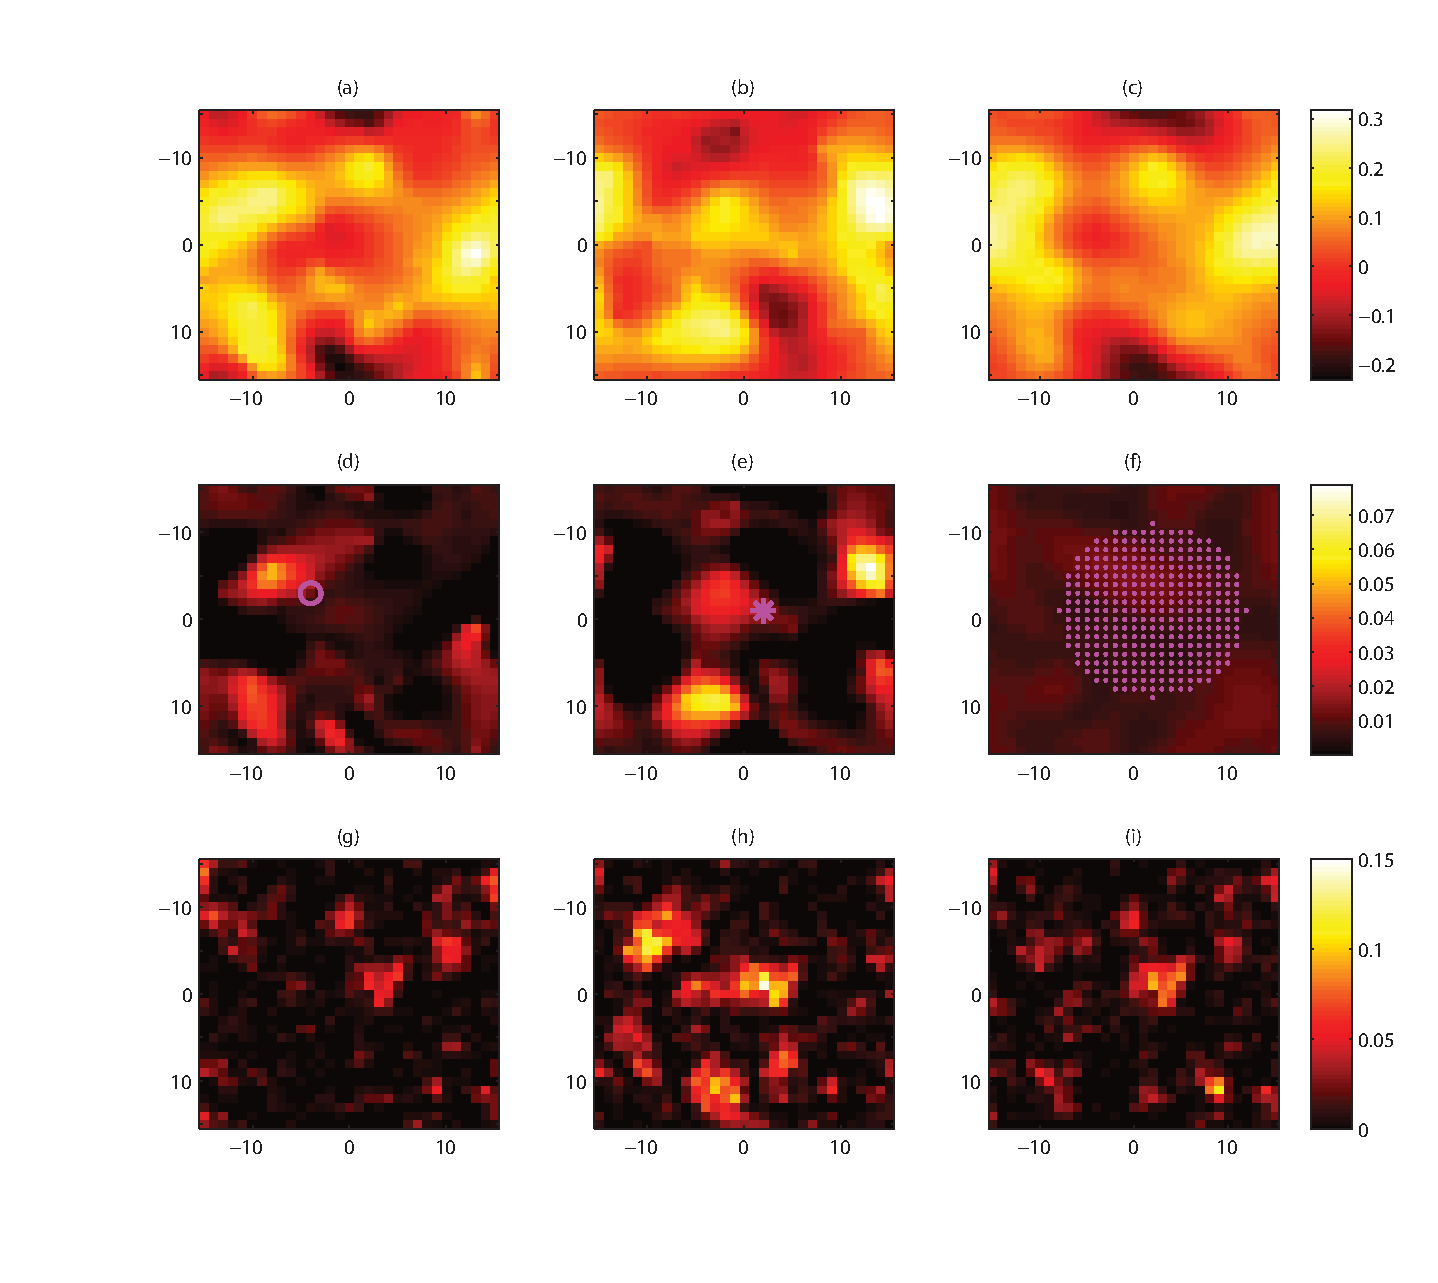
\includegraphics[trim = 30mm 20mm 2mm 2mm, width=2 \columnwidth]{firstresult.eps}%
\caption{The prediction results of Cases~$1$, $2$, and $3$ at time $t=100$ are shown in the first, second, third columns, respectively. The first, second, and third rows correspond to the prediction, prediction error variance, and squared empirical error fields between the prediction and true fields. 
True, noisy, and probable sampling positions are shown in circles, stars, and dots, respectively. The x and y axis represent 2-D localization, and colors represent the value of the desired quantity in the locations.}
\label{fig:comparelocalization}%
\end{figure*}

\begin{figure}[tb]\centering
 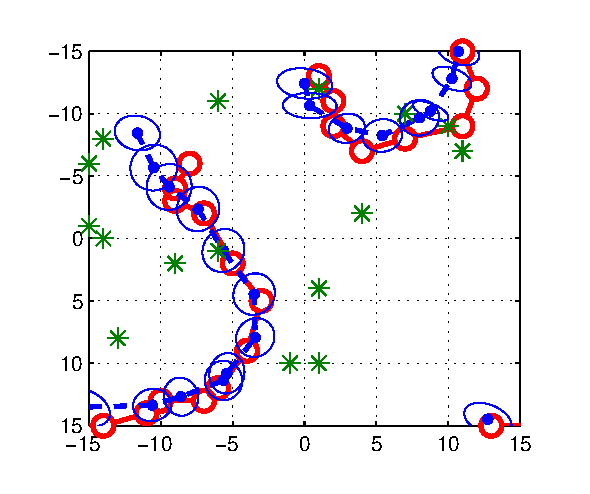
\includegraphics[trim = 0mm 5mm 0mm 2mm, width=0.95\columnwidth]{trajectory3.eps}
 \caption{The trajectories of true, predicted, and noisy sampling positions of the robot are shown by red diamonds, blue dots, and green stars for time $t \in \set{10,11, \cdots, 30}$. The blue ellipsoids show the confidence regions of about $68\%$ for the estimated sampling positions.}
 \label{fig:true}
\end{figure}

%
In this example, the fixed running time using Matlab R2009b (MathWorks) on a PC (3.2 GHz Intel i7 Processor) is about  {40} seconds for each iteration of time which is fast enough for real world implementation. 





\section{THE BODY OF THE ARTICLE}

\subsection{Mathematics} \textsf{asjcauth.cls} makes the full
functionality of \AmS\/\TeX\ available. We encourage the use of
the \verb"align", \verb"gather" and \verb"multline" environments
for displayed mathematics.

\subsection{Two wheel robot model}

Call ${q}_{ci}$, ${\theta}_{i}$ are current position and orientation of the robot. ${v}_{ci}$ and ${\omega}_{i}$ are linear and angular velocity.
\begin{equation}
	\begin{split}
		&\dot{q}_{ci}=\left[
			\begin{array}{c}
			v_{ci}\cos(\theta_{i})\\
			v_{ci}\sin(\theta_{i})\\
			\end{array}
		\right],\\
		&\dot{\theta}_{i}=\omega_{i}
	\end{split}
\end{equation}
With
\begin{equation}
\mathbf{\dot{q}_{ci}}=\left[
		\begin{array}{c}
			v_{cx}\\
			v_{cy}\\
		\end{array}
	\right]
\end{equation}
Combining (1) and (2), we have: 
\begin{equation}
	\left[
		\begin{array}{c}
			v_{cx}\\
			v_{cy}\\
		\end{array}	
	\right]=
	\left[
		\begin{array}{cc}
			\cos(\theta_{i})&{0}\\
			\sin(\theta_{i})&{0}\\
		\end{array}		
	\right]
	\left[
		\begin{array}{c}
			v_{ci}\\
			\omega_{ci}\\
		\end{array}		
	\right],
\end{equation}
Where $v_{cx}$ and $v_{cy}$ are velocity of the center point of the robot in \textit{x-axis} and \textit{y-axis} of the \textit{global coordinate}. 
Calling:
\begin{equation}
{M}(\theta)=\left[\begin{array}{cc}
			\cos(\theta_{i})&{0}\\
			\sin(\theta_{i})&{0}\\
		\end{array}
		\right]
\end{equation}

In the discrete domain, we have: 
\begin{equation}
	\frac{q_{i}(t+1)-q_{i}(t)}{\Delta{t}}=
	{M}(\theta)\left[
		\begin{array}{c}
			v_{ci}\\
			\omega_{ci}\\
		\end{array}
	\right]
\end{equation}
Thus, 
\begin{equation}
	q_{i}(t+1)=q_{i}(t)+\Delta{t}M(\theta)\left[
		\begin{array}{c}
			v_{ci}\\
			\omega_{ci}\\
		\end{array}
		\right],
\end{equation}
\begin{equation}
\theta_{i}(t+1)=\theta_{i}(t)+\Delta{t}\omega_{i}(t)
\end{equation}
On other hand, call $v_{l}$ and $v_r$ are velocity of the left and right wheels of the robot, correspondingly, we have: 

\begin{equation}
	\begin{split}
		v_{ci}=\frac{v_l+v_r}{2} \\
		\omega_{ci}=\frac{v_l-v_r}{d_{w}}\\ 
	\end{split}
\end{equation}
With $d_{w}$ is the distance between two wheel.So: 
\begin{equation}
\left[
	\begin{array}{c}
		v_{ci}\\
		\omega_{ci}\\
	\end{array}
\right]=
\left[
	\begin{array}{cc}
		\frac{1}{2}&\frac{1}{2}\\
		\frac{1}{d_{w}}&\frac{-1}{d_{w}}\\
	\end{array}
\right]
\left[
	\begin{array}{c}
		v_l\\
		v_r\\
	\end{array}
\right]
\end{equation}
Shown in Figure 2 is the diagram for the two wheel mobile robot.

\begin{figure}
\centering
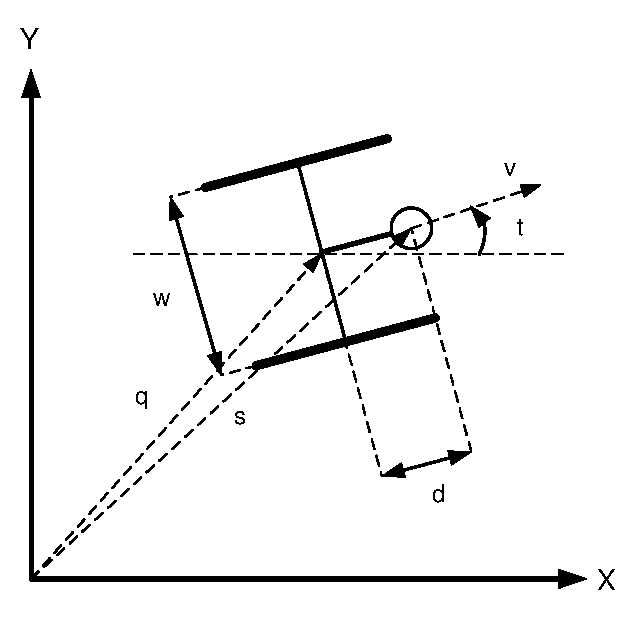
\includegraphics[width=.7\columnwidth]{Robot_kinematics.eps}
\caption{Robot's Kinematics}
\end{figure}

\subsection{Experiment setup}
\subsubsection{Mobile robot}

The mobile robot is depicted in Figure 3. The Arduino Mega board is used as the micro-controller, two wr703n router are used, one for streaming the video recorded from the web-cam equipped with paranormal lens, the other for receiving command remotely via the Internet. The overall control scheme is elaborated in Figure 4. There are three data collecting processes:
\begin{itemize}
\item The command sent to the Arduino board from the user is harvested at sampling time set to 50 milliseconds. However, due to the poor performance of the Arduino board, the actual sampling time fluctuates from 59 to 62 milliseconds. Thus,collapsing time between two samplings are recorded to be used in the simulation part.
\item The scene recorded by the paranormal web-cam is streamed on-line via the router, which can be accessible by the IP address of the router. The control program running in the control PC records the stream with 5 frame per second, e.g. 5 Hz.
\item The location of the mobile robot is tracked by the ceiling camera, by which it is updated with the same sampling rate as the streaming video.   
\end{itemize}

\begin{figure}
\centering
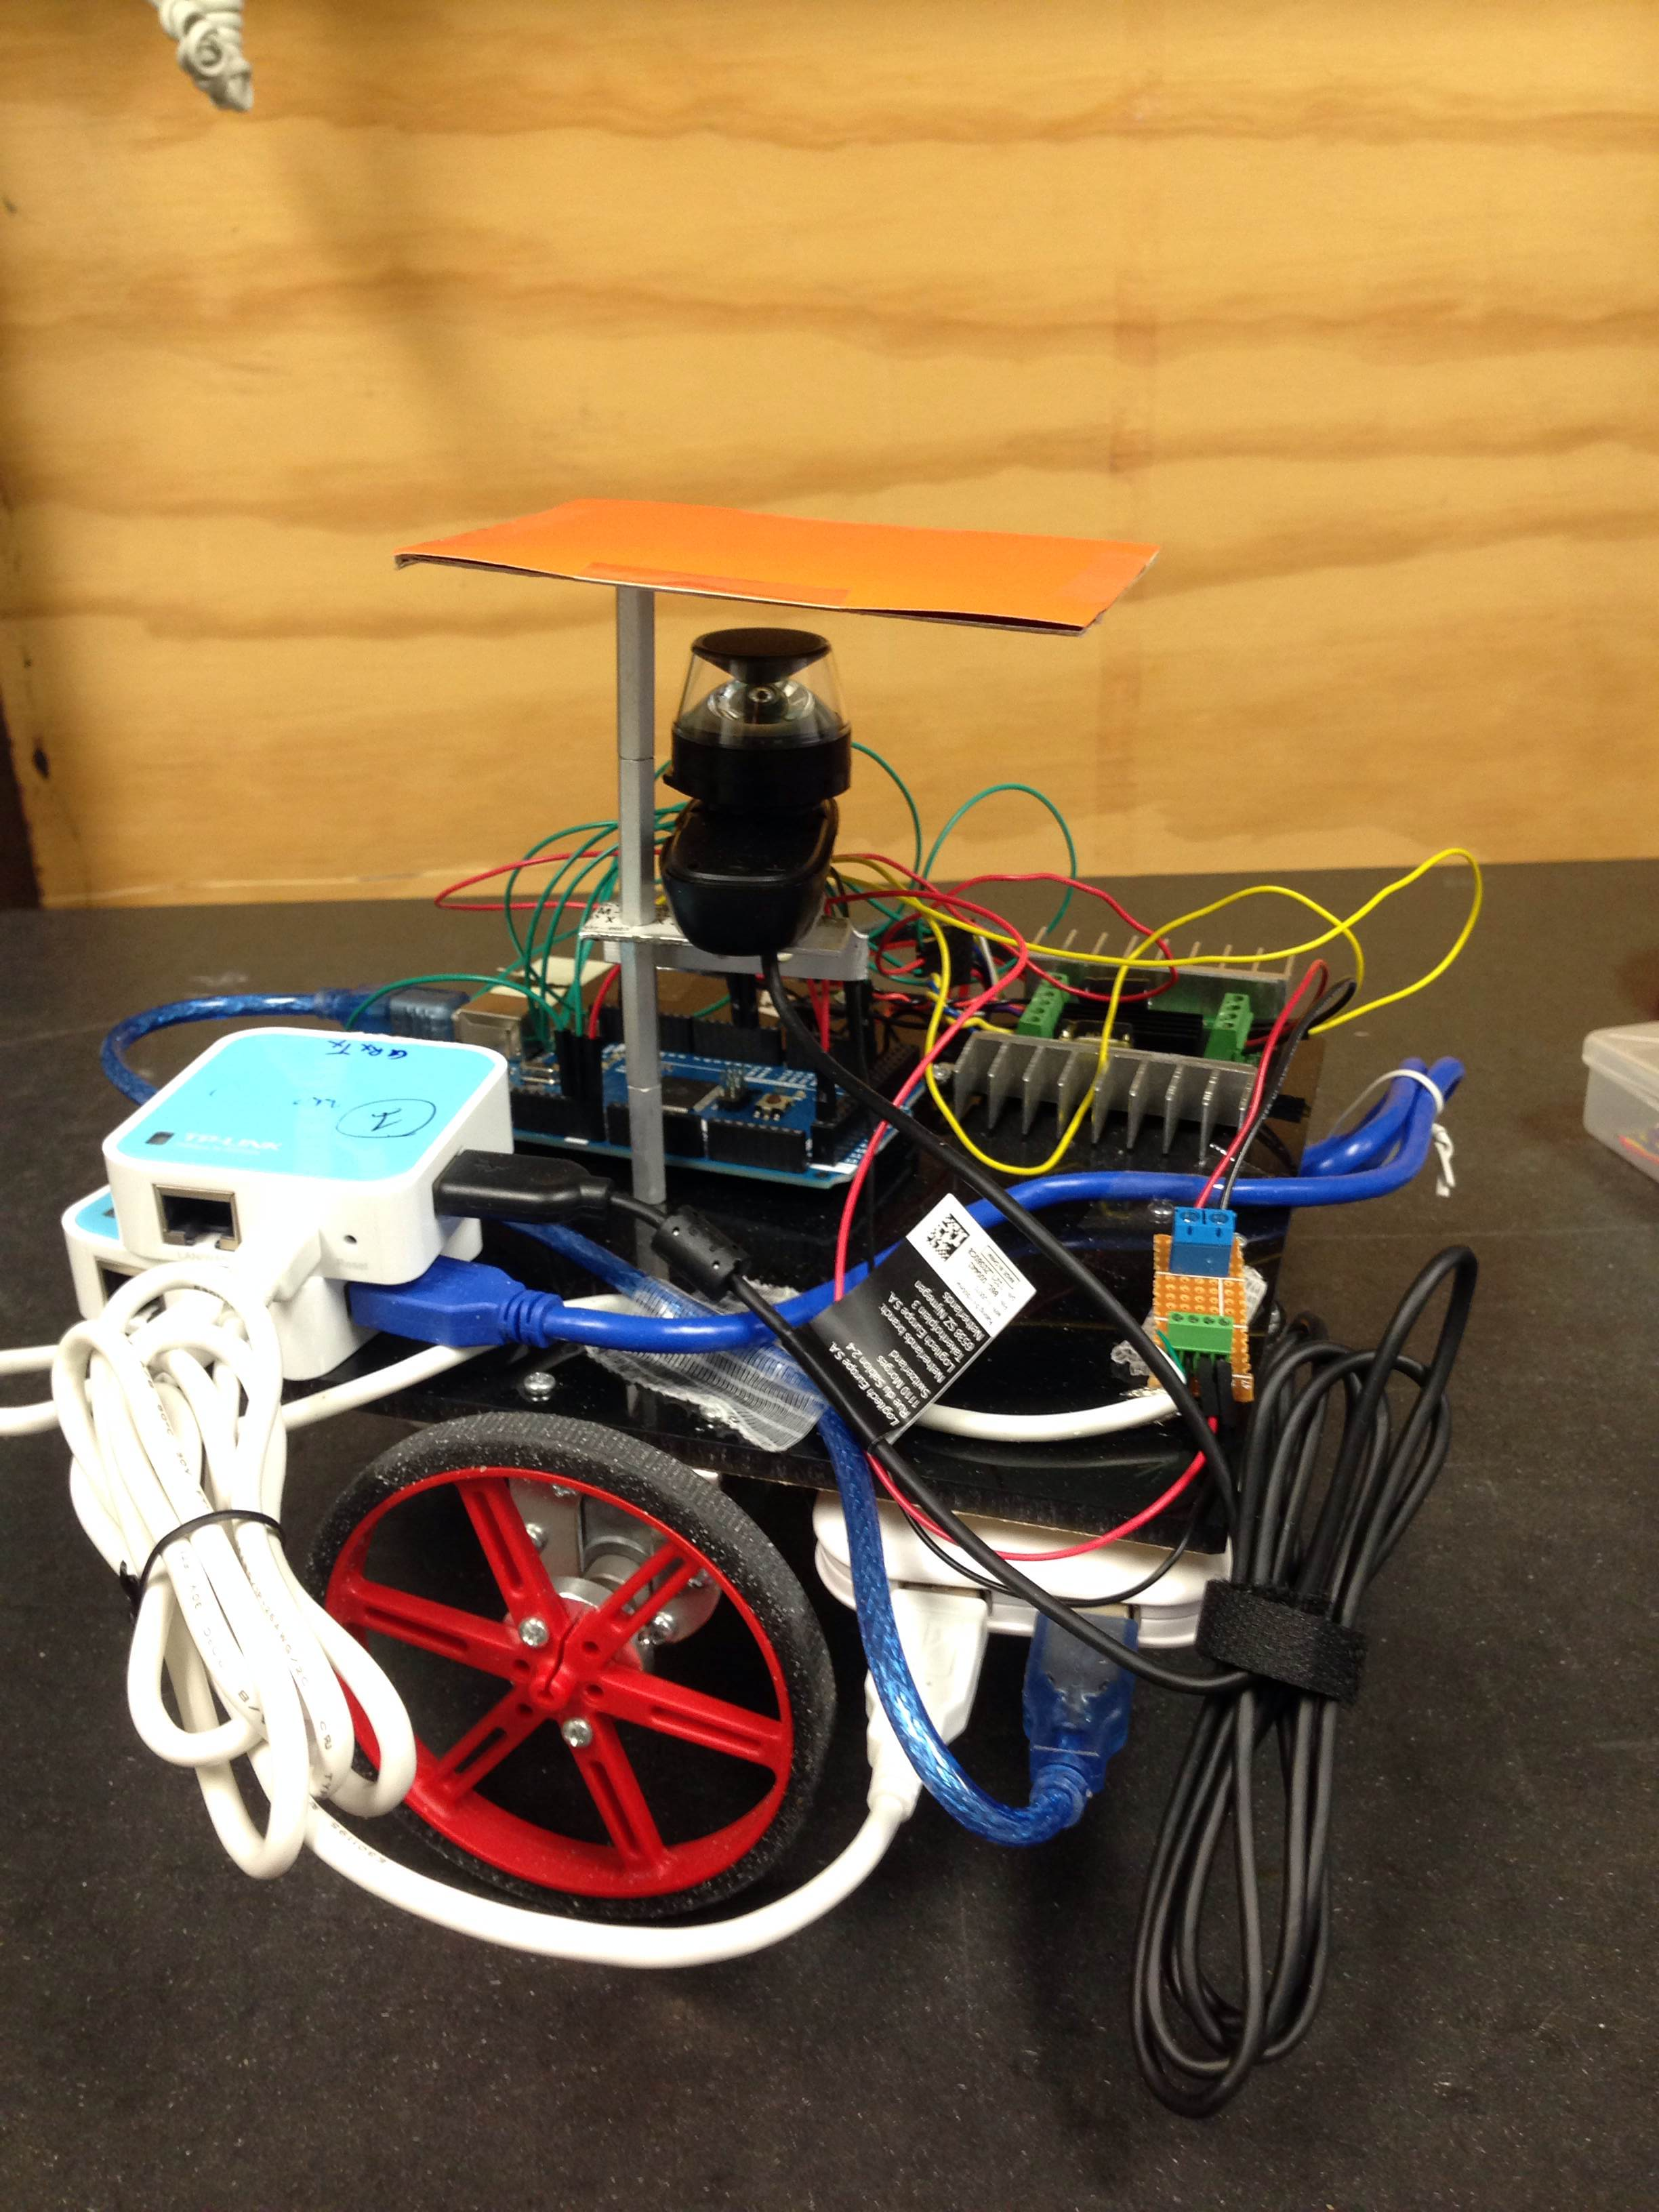
\includegraphics[width=.7\columnwidth]{mobileRobot.jpg}
\caption{Mobile Robot}
\end{figure}

\begin{figure}
\centering
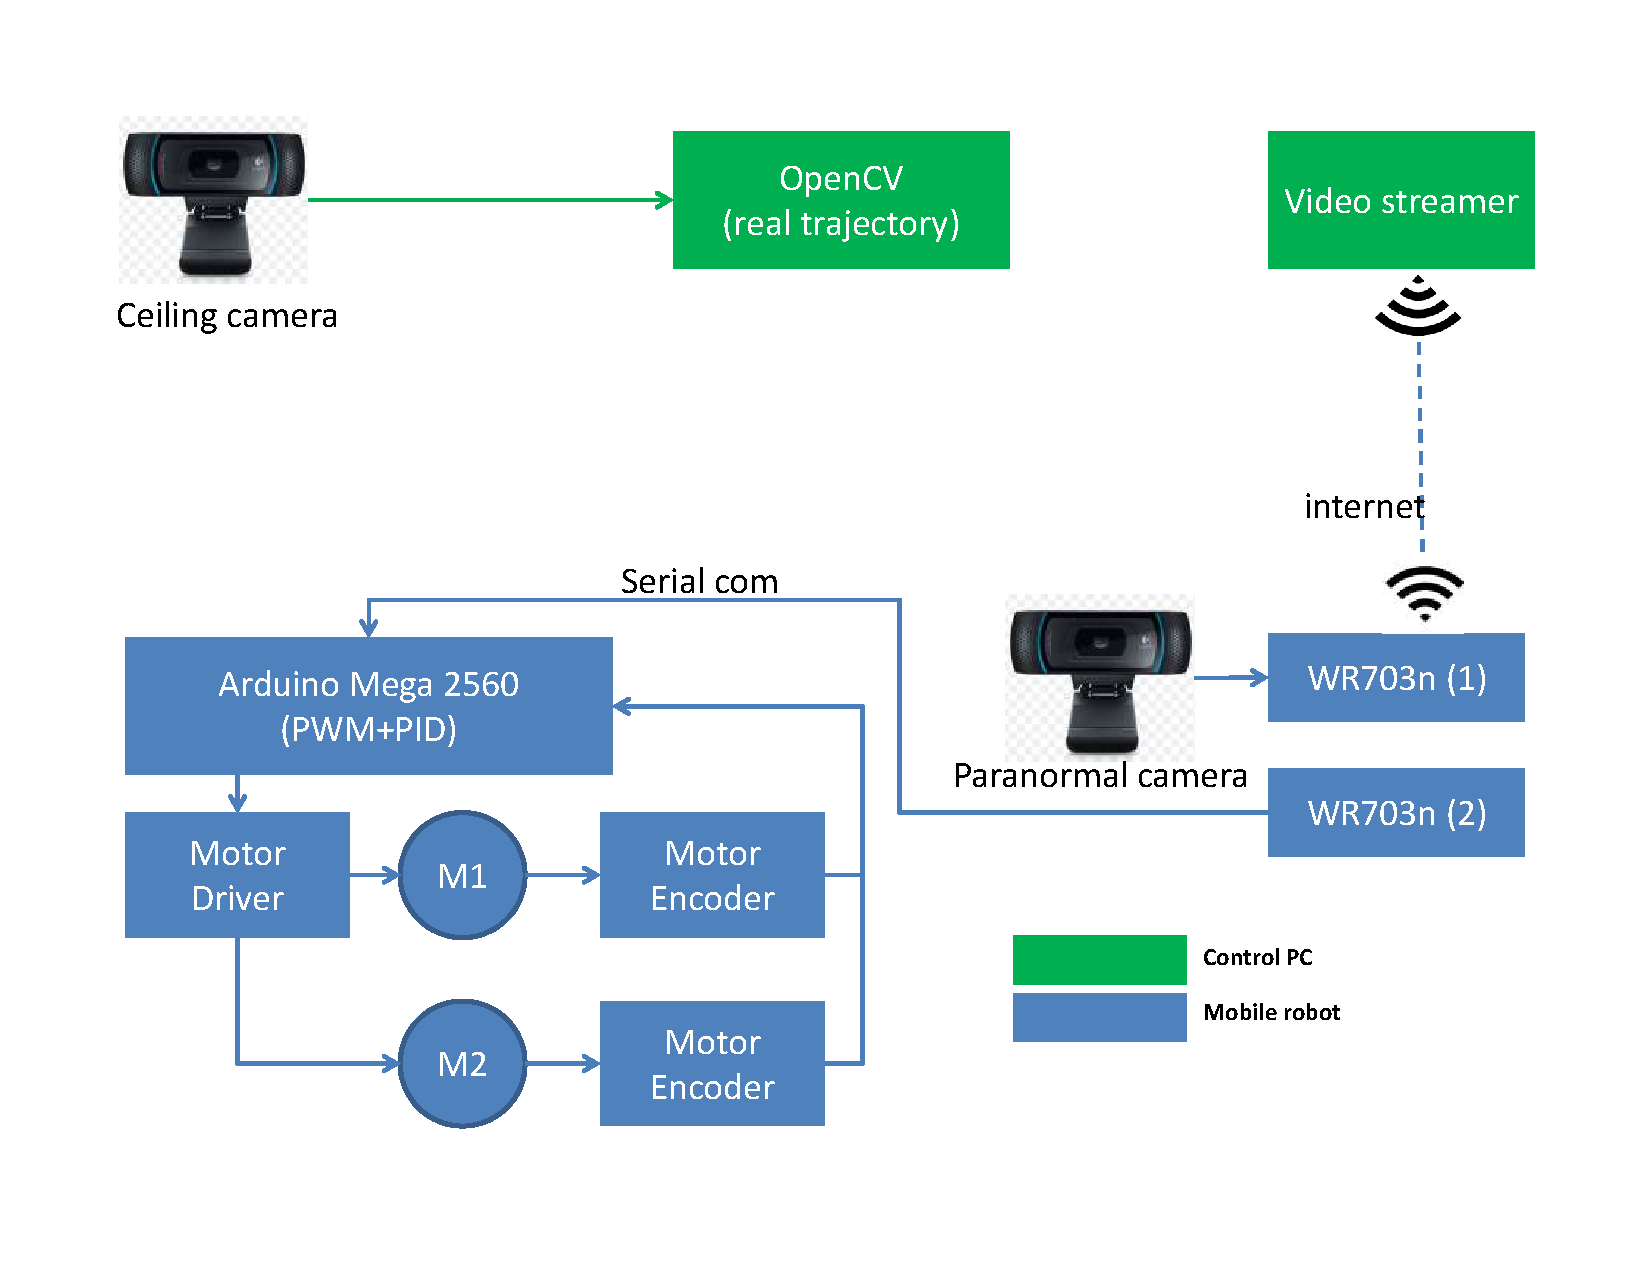
\includegraphics[width=.7\columnwidth]{ControlFlow.pdf}
\caption{Overall Control Scheme}
\end{figure}

\subsubsection{Experiment environment}
The testing environment is depicted in Figure 5. Robot is controlled in opened-loop manner by user, while the paranormal recording the surrounding scene.Two PCs are used in the experiment, one for sending command signals to the robot, the other for processing the images from the ceiling camera for tracking robot's trajectory, and recording the scene streamed from the paranormal camera installed on the robot. 

\begin{figure}
\centering
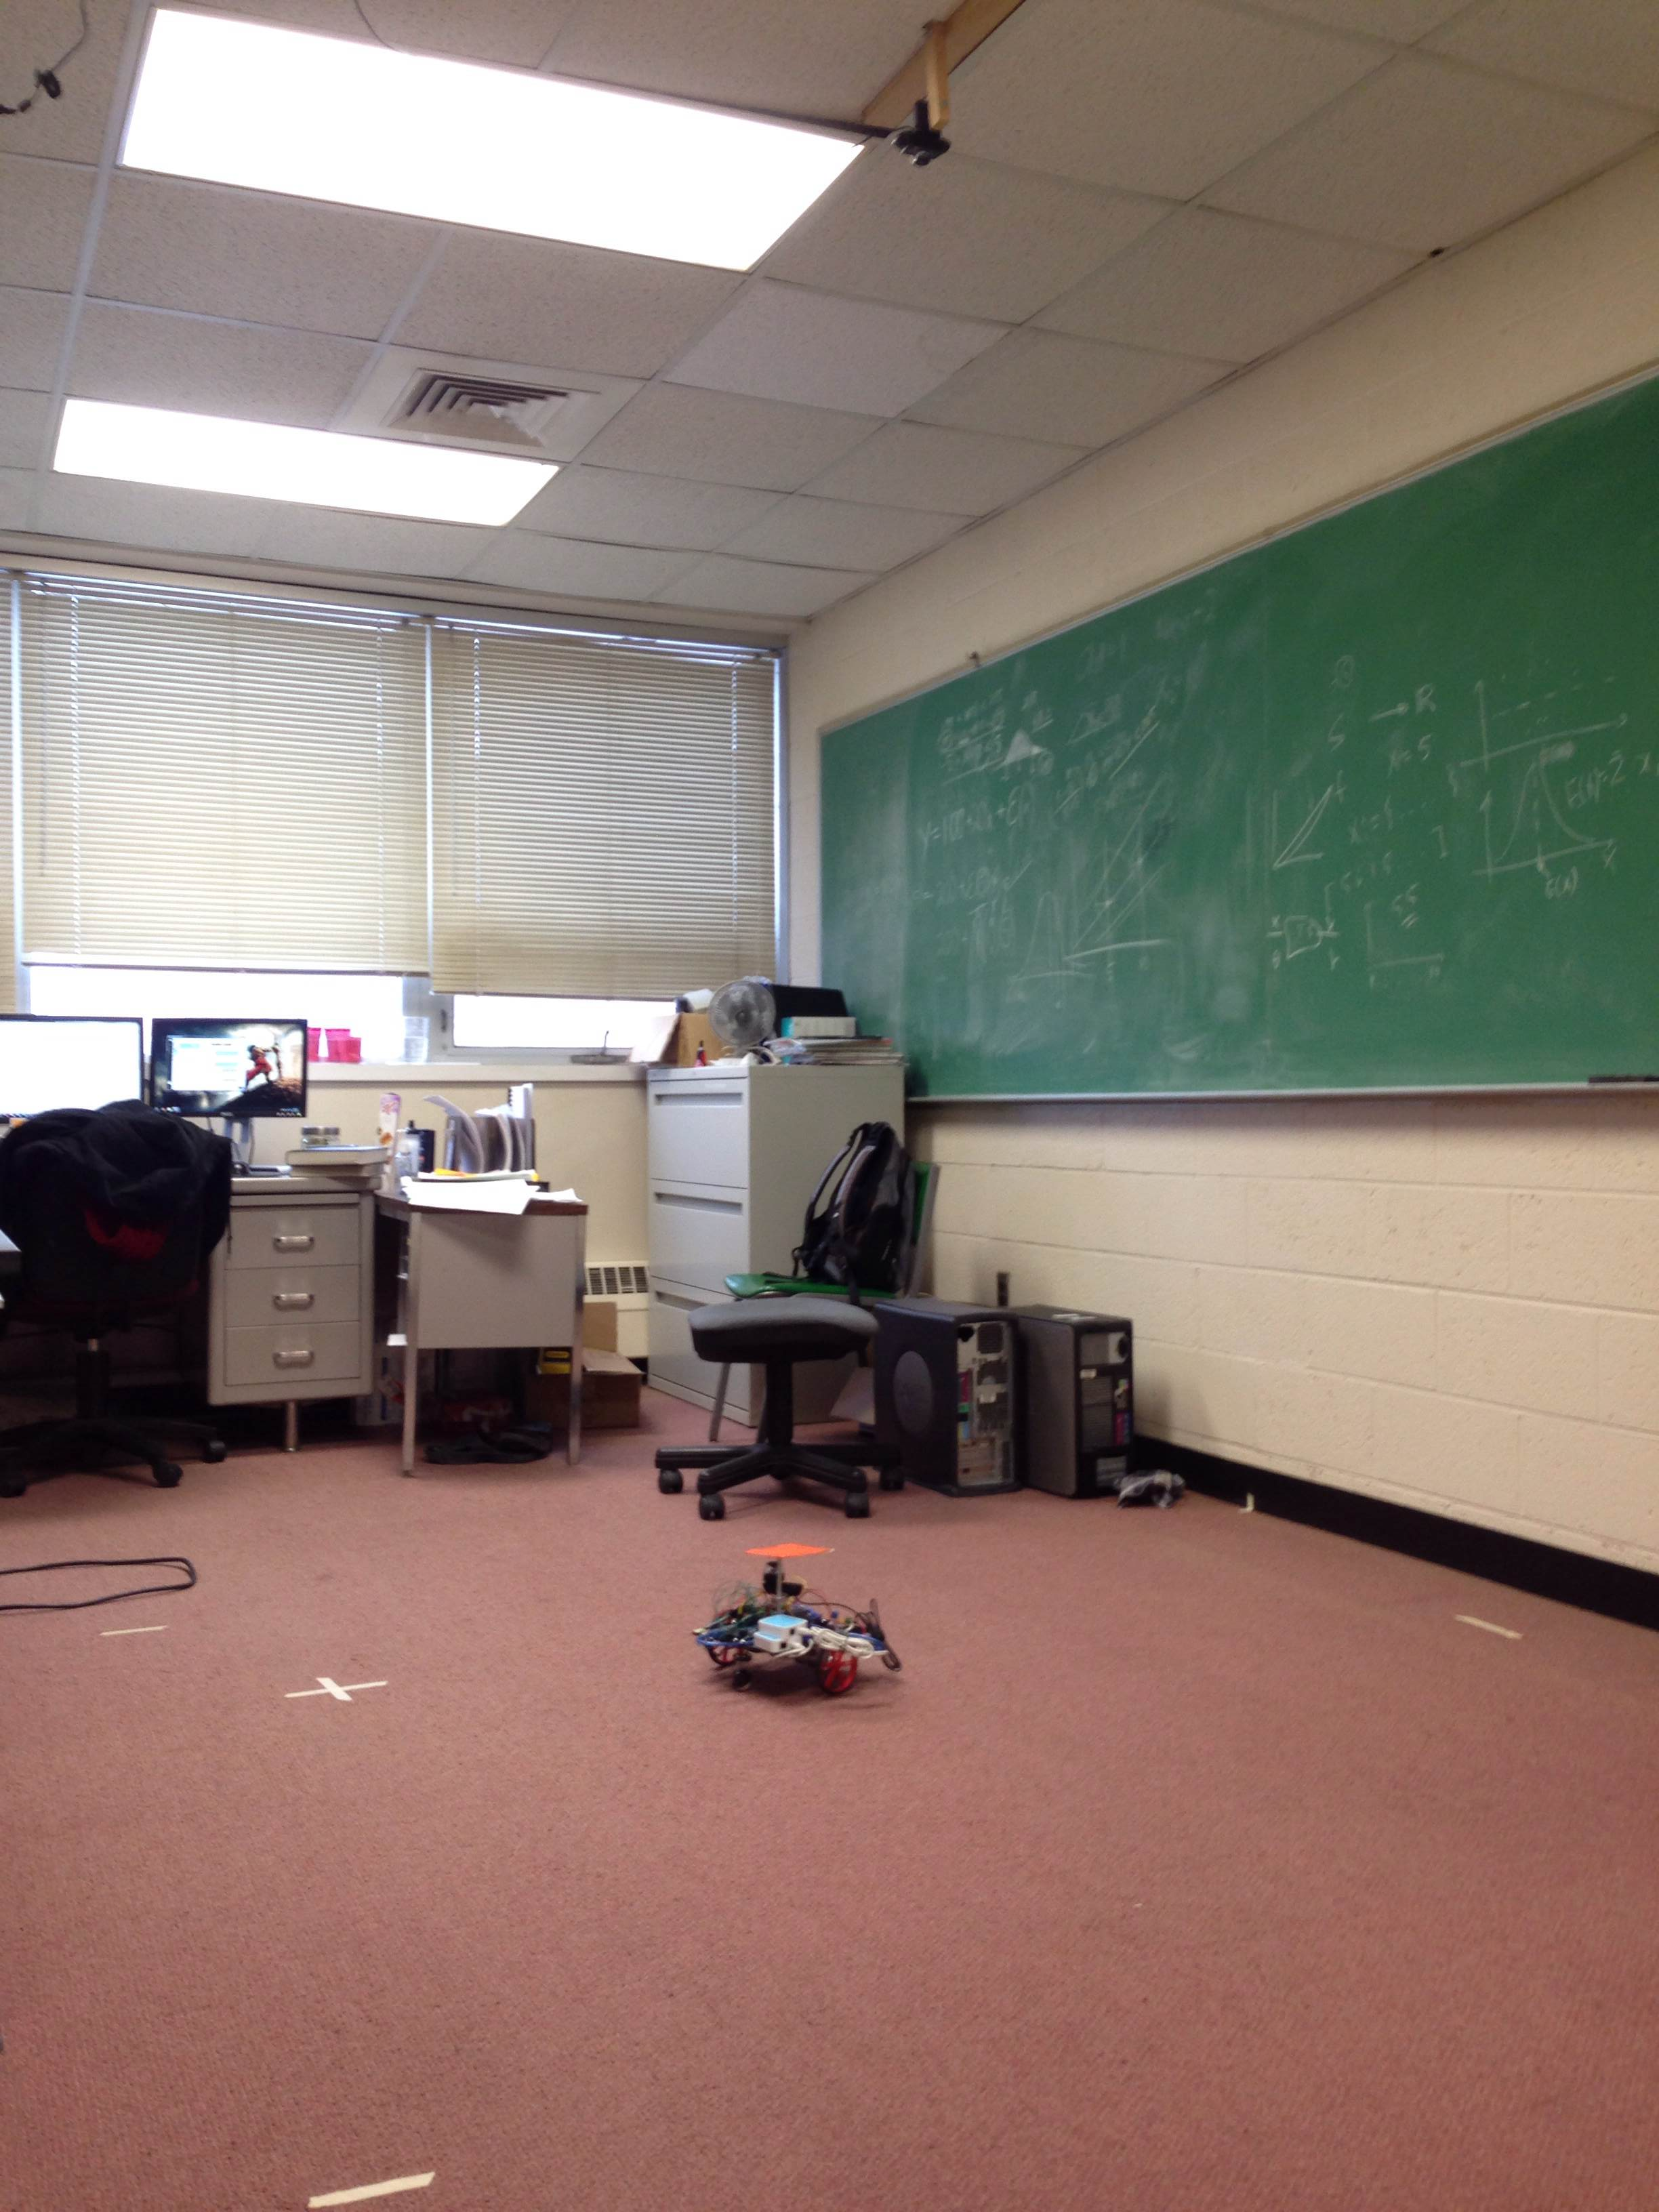
\includegraphics[width=.7\columnwidth]{testingEnvironment.jpg}
\caption{Testing Environment}
\end{figure}

\subsection{mat-lab code explanation}
The command saved from the Arduino board is stored in \emph{huan} file. The real robot's trajectory \emph{in image frame coordinate} is exported in \emph{output.txt} file. The scene recorded from the paranormal camera is saved in \emph{record12115h08.avi} file.

The file \emph{robotTrackSimulation.m} simulates the robot model which is described in 5.1. The simulated result is converted to the coordinate in picture's frame by the camera matrix stored in the file \emph{calibmatrix.mat}. The trajectory then is processed through a second calibration by translation and scaling matrices to minimize the difference between the simulated and the real trajectory. The model is confirmed when the distance is sufficiently small.

The frames are queried from the video in the file \emph{frameQuery.m}. The experiment is executed in 112 seconds, e.g. sum of the sampling time from the command file and the length of the video is exactly matched. The command is sampled with 60 milliseconds sampling time, so there are 1852 sample points, which in turn are sub-sampled by factor of 1:4. Thus, there are \textbf{463} sub-sampling points. The video is recorded with 5 fps, so there are \textbf{558} frames for the video in total. The frames are numbered from 1 to 558. The sub-sampled command input is stored in the \textbf{commandSS} variable which is 463x3 matrix. The first two columns are the command input of linear velocity and angular velocity for the robot, correspondingly, the final column is exact time when a command was sent, in the time-line from 0 to 112.5 second. The variable \textbf{outPut} contains the real coordinate of the robot, sampled with frequency of 5Hz.  

The frames and the sub-sampled command are matched in following manner:

The time (in second) for each sample point in 463 sample points of the command is calculated in the time-line from 0 to 111 second, then it is projected to the frames set by following equation:

\begin{equation}
frame number=time\times\frac{558}{111}
\end{equation}  

The 463 sample frames are save in the \emph{frames} folder.



\section{Conclusion}
In this paper, we provide an approximate Bayesian solution to the problem of simultaneous localization and spatial prediction (SLAP), taking into account kinematics of robots and uncertainties in the precision matrix, the sampling positions, and the measurements of a GMRF in a fully Bayesian manner. In contrast to \cite{jadaliha2012efficient}, the kinematics of the robotic vehicles are integrated into the inference algorithm. The simulation results show that the proposed approach estimates the sampling positions and predicts the spatial field along with their prediction error variances successfully, in a fixed computational time.
The simulation study suggests that the complexity of the proposed scalable inference algorithm is affordable for a robot to operate in real world situations.


\section{Acknowledgement}
This work has been supported by the National Science Foundation through CAREER Award
CMMI-0846547. This support is gratefully acknowledged.

%
%\section{Appendix}
%Recall that the probability density function of sum of two random variables is obtained from the following formula.
%\[
%		\f{X+Y}{\alpha} = \int{\f{X}{\beta}\f{Y}{\alpha-\beta} d\alpha}.
%\]
%
%The law of total variance says
%\[
%\Cov\left(Y\right) = E \left( \Cov\left(Y|X\right)\right) + \Cov \left( E\left(Y|X\right)\right).
%\]
%In this law, the inner expectation or covariance is taken with respect to $Y$ conditional on $X$, while the outer expectation or covariance is taken with respect to $X$. The overall covariance of $Y$ is summation of two components as follows.
%\begin{itemize}
%	\item the average of the covariance of $Y|X$, as $X$ varies;
%	\item the covariance of the average of $Y|X$, as $X$ varies.
%\end{itemize}

% ------------------------------------------------------------------------

\bibliographystyle{IEEEtran} \bibliography{reference}

\end{document}
